\ifnum\aluno=1
\renewcommand\chapterillustration{./abertura-combinatoria}
\else
\renewcommand\chapterillustration{./abertura-combinatoria-professor}
\fi

\renewtcolorbox{openningbox}{
  enhanced,
%  jigsaw,
  opacityframe=.3,
  opacityfill=.3,
  width=105mm,
  left=3mm,
  right=3mm,
  top=3mm,
  bottom=.5mm,
  colback=white,
  colframe=white,
  arc=3mm,
  sharp corners=uphill,
    % frame empty,
    % arc = 8pt,
    lower separated = false,
    before upper = \tcbsubtitle{O QU\^E?},
    before lower = \tcbsubtitle{POR QU\^E?},
    fontupper = \sffamily,
    fontlower = \sffamily,
    sharp corners = north,
    subtitle style = {
      frame empty,
      fontupper = \fontsize{13pt}{0}\selectfont\titlefont\bfseries,
      colback = cor1,
      coltext = black!70,
      width = 3.5cm,
      arc = 8pt,
      rounded corners = east
    }
  }

\makeatletter
\ifnum\aluno=1
\else
\renewcommand*{\toclevel@section}{1}
\renewcommand*{\toclevel@subsection}{4}
\renewcommand*{\toclevel@paragraph}{5}
\renewcommand*{\toclevel@subparagraph}{6}

\renewcommand*{\toclevel@exploresec}{2}
\renewcommand*{\toclevel@practicesec}{2}
\renewcommand*{\toclevel@arrangesec}{2}
\renewcommand*{\toclevel@knowsec}{1}
\renewcommand*{\toclevel@exercisesec}{1}

\setcounter{tocdepth}{2}
\fi
\makeatother


\renewcommand\chapterwhat{Problemas do cotidiano que envolvam o processo de contagem. Começando com a contagem de conjuntos de dados que podem ser enumerados e organizados em tabelas, árvores e/ou $n-$uplas, seguindo para a compreensão da necessidade do uso do  Princípio Multiplicativo e do Princípio Aditivo para solução de problemas combinatórios mais gerais.}
\renewcommand\chapterbecause{
Problemas de contagem estão presentes em várias situações do cotidiano, como por exemplo, a quantidade de senhas de um determinado padrão. Uma senha eficiente é aquela difícil de ser descoberta então quanto maior o número de senhas de um determinado padrão melhor se torna a segurança da senha criada. Outros exemplos são: quantidade de placas de automóveis; quantidade de dígitos em números de telefones; quantidade de jogos possíveis na loteria, quantidade de números de IP's (do inglês \textit{Internet Protocol}), escalas de trabalhos ou de aulas, etc. Combinados com o estudo de Probabilidade ajudam na tomada de decisão, ao ponto que fornecem as possibilidades de  ocorrência de determinados fatos. 

Problemas de contagem também estão presentes em outras áreas do conhecimento como Física, Biologia e Computação. Além disso, o raciocínio combinatório desenvolve características importantes na resolução de problemas de maneira geral como processos de reflexão e abstração, levantamento de hipóteses, escolha de caminho para a solução e construção de generalizações, processos de investigação, de construção de modelos, formulação e a testagem de conjecturas; enfim, resolução e elaboração de problemas recorrendo a estratégias diversas, habilidades gerais presentes na BNCC.} 
\chapter{Análise Combinatória}
\label{combinatoria-chap}

\mbox{}\thispagestyle{empty}\clearpage

\thispagestyle{empty}

\begin{center}
Projeto: LIVRO ABERTO DE MATEMÁTICA

\noindent \begin{tabular}{lcccr}

\includegraphics[scale=.15]{impa}& \quad\quad& 
\includegraphics[width=3cm]{logo} & \quad\quad& 
\includegraphics[scale=.24]{obmep} 
\end{tabular}
\end{center}

\vspace*{.3cm}

Cadastre-se como colaborador no site do projeto: \url{umlivroaberto.org}



% \begin{center}
%   \includegraphics[width=2cm]{canvas}
% \end{center}

\begin{tabular}{p{.15\textwidth}p{.7\textwidth}}
Título: & Análise Combinatória\\
\\
Ano/ Versão: & 2020 / versão 0.1 de \today\\
\\
Editora & Instituto Nacional de Matem\'atica Pura e Aplicada (IMPA-OS)\\
\\
Realização:& Olimp\'iada Brasileira de Matem\'atica das Escolas P\'ublicas (OBMEP)\\
\\
Produção:& Associação Livro Aberto\\
\\
Coordenação: & Fabio Simas, \\
			&  Augusto Teixeira (livroaberto@impa.br)\\
\\
  Autores: & Carlos A. Gomes (UFRN),\\
             & Lhaylla Crissaff (UFF).\\
        
\\
Colaboração: & \\
\\
Revisor: &  \\
         &  \\
\\
Design: & Andreza Moreira (Tangentes Design) \\
\\
  Ilustrações: & --- \\ 
\\
Gráficos: & ---\\
\\
  Capa: & Foto de James Sutton, no Unsplash \\
  		& https://unsplash.com/photos/qXn5L9BqRbE \\

\end{tabular}
\vspace{.5cm}



\begin{figure}[b]
\begin{minipage}[l]{5cm}
\centering

{\large Licença:}

  
\includegraphics[width=3.5cm]{cc-by-nc-sa}
\end{minipage}\hfill
\begin{minipage}[c]{5cm}
\centering
{\large Desenvolvido por}


\includegraphics[width=2.5cm]{logo-associacao.jpg}
\end{minipage}
\begin{minipage}[r]{5cm}
\centering

{\large Patrocínio:}
  \vspace{1em}
  
\includegraphics[width=3.5cm]{itau}
\end{minipage}
\end{figure}

\mainmatter

\begin{apresentacao}{Introdução}
\subsection{Objetivos gerais}
\begin{itemize}
\item Reconhecer situações do cotidiano nas quais as técnicas elementares de contagem são efetivas; 
\item Entender a importância da organização dos dados para contagem adequada; 
\item Aplicar os princípios aditivo e multiplicativo na resolução das situações problema e na construção das generalizações; 
\item Avaliar se as soluções encontradas realmente satisfazem as exigências do problema.
\end{itemize}

\paragraph{Habilidades da BNCC}

\begin{habilities}{EM13MAT310}
Resolver e elaborar problemas de contagem envolvendo diferentes tipos de agrupamento de elementos, por meio dos princípios multiplicativo e aditivo, recorrendo a estratégias diversas, como o diagrama de árvore.
\end{habilities}

\paragraph{Em que contexto?}

Situações do dia a dia tais como entender porquê é seguro utilizar senhas com muitos dígitos ou quantos caminhos diferentes podemos fazer de um ponto a outro, situações do cotidiano escolar, e temas de interesse dos adolescentes que:

\begin{itemize}

\item sejam possíveis de serem resolvidos utilizando os Princípios Aditivo e Multiplicativo;
\item mostrem a importância da organização dos dados e das ações para contagem correta;
\item permitam a comparação com problemas já estudados;
\item deixem claro a importância de se dividir um problema complexo em problemas menores;
\item diferenciem quando objetos são distintos ou não e quando a ordem das escolhas muda ou não o agrupamento a ser contado;
\item auxiliem nas generalizações.

\end{itemize}

\paragraph{Distratores}

Os problemas de contagem podem ter vários caminhos de resolução e um valor numérico grande, o que dificulta a conferência da solução. Algumas pesquisas apontam distratores (erros mais comuns) cometidos durante o processo de aprendizagem deste conteúdo, mas não apresentam soluções para sanar estes erros. Acreditamos que adotar medidas como organização de dados, diagramação  e divisão em casos menores pode diminuir as dificuldades enfrentadas por estudantes. Também entendemos que a categorização dos problemas em permutação, arranjo e combinação não facilitam a compreensão em um contato inicial com o assunto, por isso sugerimos a utilização de fórmulas apenas depois de bem compreendidos o Princípio Aditivo e o Princípio Multiplicativo. 

Segue listado abaixo uma relação de distratores no ensino de Análise Combinatória :


\begin{enumerate}
\item \textbf{Listagem não sistemática:} os alunos realizam a listagem sem nenhum tipo de organização. Dessa maneira, a listagem de possibilidades pode ficar faltando elementos, ou com elementos em excesso; 
\item \textbf{Ordem dos elementos: }os alunos não percebem a característica do problema com relação à ordem dos elementos, considerando a ordem relevante em problemas que não é, e desconsiderando-a quando é necessária levar em conta. Um dos erros que pode surgir é a classificação de um problema de combinação como um problema de arranjo, e vice-versa. 
\item \textbf{Repetição dos elementos:} os alunos não percebem a característica do problema em relação à possibilidade de repetição de elementos.  Então, desconsidera a repetição dos elementos quando o problema permite, assim como o inverso, considerando a repetição dos elementos em um problema que não permite repetição. 
\item \textbf{Diferenciação dos problemas combinatórios:} alunos possuem dificuldades nos conceitos de cada tipo de problema de combinatória, classificando os problemas de maneira errônea;
\item \textbf{Utilização das fórmulas:} além das dificuldades de lembrar as fórmulas de cada problema, os alunos apresentam dificuldades na substituição dos valores do problema na fórmula e resolvê-la;
\item \textbf{Utilização do diagrama de árvores:} os alunos montam o diagrama de árvores com uma estrutura errônea; 
\item \textbf{Interpretação:} inicia-se do princípio de que as dificuldades dos alunos estão principalmente na confusão sobre a relevância da ordem dos elementos, na falta de organização para enumerar os dados sistematicamente, dúvidas na identificação da operação aritmética equivalente e interpretação incorreta do problema, quando este apresenta mais de uma etapa.
\item \textbf{Contagem de Agrupamentos:} os estudantes nem sempre compreendem que os problemas de combinatória se referem a contagem de todos os agrupamentos possíveis e não a divisão do total de elementos pelo número de elementos no agrupamento.
\end{enumerate}

Este material pretende construir os conceitos fundamentais para os problemas de contagem:  Princípio Aditivo e Princípio Multiplicativo, utilizando a resolução e elaboração de problemas envolvendo os vários tipos de agrupamentos existentes, e recorrendo a várias abordagens de representação.  Os conteúdos estudados necessitam que os estudantes  saibam como pré-requisitos as quatro operações básicas: adição, subtração, multiplicação e divisão. 
 
O livro adota como metodologia a investigação em sala de aula através da resolução de problemas, \cite{Ponte}. As seções foram escritas para que o estudante desenvolva o raciocínio sobre os Princípios Fundamentais por meio de atividades investigativas, iniciando na primeira seção com atividades  sem uso de nomenclatura específica e com problemas pequenos para que seja possível listar as possibilidades e pensar em critérios de organização. Na segunda seção várias tipos de problemas são apresentados, sem estarem separados pelos agrupamentos convencionais, de modo que seja possível construir novo conhecimento por pequenas variações nos problemas já estudados. A terceira seção se refere a organização dos agrupamentos convencionais: permutação, arranjo e combinação, não é uma seção obrigatória, por entender que é de fácil compreensão por parte de um estudante que tenha realizado e discutido as seções anteriores.
 
Cada atividade é composta de vários itens que devem ser propostos ao estudante na ordem dada. Assim como a ordem dada nas atividades de cada seção.  Os itens e sua ordem foram pensados para a construção do raciocínio combinatório do estudante.
 
Uma característica deste material é a não apresentação de fórmulas de contagem aos estudantes. No ensino usual de Análise Combinatória o uso de fórmulas é peça chave para o desenvolvimento dos exercícios. No entanto, ao passo que essas notações tornam as contas mais facies, entender qual é a fórmula certa, ou ainda, de que agrupamento o problema trata, se torna um distrator, como aponta pesquisas que destacam dificuldades dos estudantes. Discussões sobre a classificação em permutação, arranjo ou combinação se tornam o foco das aulas, o que acreditamos não ser essencial para a construção do raciocínio combinatório. Na maioria dos casos, uma fórmula sozinha não é suficientes para resolver os problemas.
  
 No entanto, a falta de fórmulas faz com que este material não se caracterize como um livro texto ao estudante com estratégias e respostas diretas  em  cada questão, muito menos tem intenção de  classificar questões em seus tipos de acordo aos agrupamento possíveis. Sendo assim é essencial para a aprendizagem interferência, mediação e exploração das respostas dos estudantes por parte do docente, em cada item das atividades. 
 
 De maneira geral é importante acolher e discutir as soluções apresentadas pelos estudantes. Todas as atividades podem ser trabalhadas individualmente, mas acreditamos que  os resultados serão melhores se os estudantes puderem trabalhar nas atividades em duplas ou pequenos grupos,  para que juntos construam uma estratégia para a solução que depois deve ser compartilhada com a turma.  No momento de compartilhar a solução será importante que percebam que não existe maneira única de organizar a contagem e apresentar as variações de possibilidades. Essa etapa é importante para a construção do raciocínio combinatório.
 
 
 As  Atividades \textbf{Calculadora Combinatória} e \textbf{Testando a Calculadora Combinatória} são propostas para que as fórmulas sejam desenvolvidas pelos estudantes acreditando ser um momento de amadurecimento para compreensão da generalização, visto que, mesmo não sendo importante ao desenvolvimento do raciocínio de contagem, as mesmas aparecem na literatura e poderão ocorrer em situações acadêmicas dos estudantes, como por exemplo o ENEM.  Aqui no material do professor as fórmulas são deduzidas e as orientações para o projeto de construção da Calculadora Combinatória são dadas. As duas atividades citadas encontram-se na seção "Para Saber Mais", por considerarmos não ser essencial para compreensão dos conceitos presentes no material e não são recomentadas pela BNCC.

As soluções apresentadas são feitas sem o uso das fórmulas, mas podem ser refeitas com o uso delas se assim desejarem. 

\end{apresentacao}


\def\currentcolor{session1}

\begin{texto}
{
  \section{Princípios Fundamentais da Contagem}
  As primeiras atividades têm o objetivo de mostrar aos estudantes a importância da organização nos processos de contagem, assim como possibilitar o uso de diferentes tipos de registros: tabelas, n-uplas e/ou árvores, que auxiliam nesse processo.  Para a solução da Atividade 4: \textbf{Desafios das colorações de mapas}  novas estratégias deverão ser pensadas, pois  o estudante deve notar que listar todos os casos se torna inviável.  Essa atividade pode ser utilizada para demonstrar a necessidade do uso do Princípio Aditivo e Princípio Multiplicativo que são as ferramentas essenciais para a construção do raciocínio combinatório.  Outro ponto importante tratado é o uso da divisão como ferramenta para retirada de repetições nos processos de contagem e a subtração para retirada de casos contados a mais.
}
\end{texto}
\begin{objectives}{Escolhendo o nome da empresa}
{
\begin{itemize}
\item Analisar a necessidade de organização dos registros para a resolução de problemas de contagem. Refletir sobre as possíveis variações de um problema e os impactos em sua solução. Construir informalmente os Princípios Aditivo e Multiplicativo. Utilizar a listagem ou árvore como representação.
\end{itemize}
}{1}{1}
\end{objectives}
\mspace{-2em}
\begin{sugestions}{Escolhendo o nome da empresa}
{
O esperado para esta atividade é que os estudantes listem as possibilidades e percebam a importância da listagem sistemática. Além disso, percebam que em algumas situações não é possível listar as possibilidades, mas novos caminhos podem ser tomados.

É importante que, se nenhum grupo percebeu a possibilidade de solução apresentada no item b), essa solução seja apresentada para a turma para resolver o item c). Eles devem perceber que uma informação prévia pode mudar a organização da solução, mas no entanto, independente do caminho escolhido a solução deve ser a mesma. Entender ambos caminhos será importante para o desenvolvimento do caso geral.

No item $d$ pode ser feito o caso geral  e introduzido o conceito de fatorial de $n$ dado por $n \cdot (n-1) \cdot 3 \cdot 2 \cdot 1= n!$.

\textbf{Tempo de Execução}: A questão pode ser feita em 30 minutos sendo utilizados para os itens \titem{a)} e \titem{b)} entre 5 a 10 minutos, e para os itens \titem{c)} e \titem{d)}, 5 minutos cada.  
}{1}{1}
\end{sugestions}
\begin{answer}{Escolhendo o nome da empresa}
{
\begin{enumerate}
\item Uma maneira seria começar pelas possibilidades que se iniciam com a letra $M$, seguidas das que iniciam com $R$ e por último as que iniciam com $I$ é possível contar todas as possibilidades sem repetição: 
                    
$$MRI, ~ MIR, ~ RMI, ~ RIM, ~ IMR, ~ IRM.$$

Uma ilustração mais usual é as possibilidades serem dispostas em colunas ou como árvore: 
$$MRI ~~ RMI~~IMR$$ 
$$MIR ~~ RIM~~IRM ,$$                     
\begin{figure}[H]
\centering

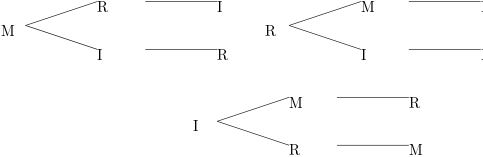
\includegraphics[scale=0.5]{grafo1.png}
\end{figure}
%quis fazer uma árvore de possibilidades                    
\item Já tendo a solução anterior é desejável que os estudantes percebam que em cada resultado apresentado no item a) é possível colocar a nova inicial em quatro posições distintas, exemplo: 
$\_ M \_ R\_ I \_ $, logo cada solução do item anterior gera 4 novas soluções para este item. O total então será $4+4+4+4+4+4= 6 \cdot 4=24$. Ou seja, não seria necessário recomeçar a organização e nem listar todos os casos. Pode ser que alguns estudantes tenham resolvido o item b) com a mesma estratégia usada no item a). Nesse caso o professor pode mediar uma discussão com os estudantes sugerindo a eles que existe outra forma. 

\item Não. Uma informação prévia pode mudar a organização da solução, mas no entanto, independente do caminho escolhido a solução deve ser a mesma. 

\item Tomando uma solução qualquer do item b) digamos $MRIL$ e a estratégia de pensar nos espaços vazios seriam $\_M\_R\_I\_L\_$,  5 espaços e a nova solução seria $24+24+24+24+24=5 \cdot 24=  120.$ para 5 letras, $6 \cdot 120= 720$ para 6 letras, $7\cdot 720=5040$ para 7 letras e $8 \cdot 5040= 40.320$ para oito letras. Fazendo o caso 2 como recomendado, é possível perceber que de maneira geral para $n$ letras 
$n \cdot (n-1) \cdot 3 \cdot 2 \cdot 1= n!$.
A solução no caso geral não precisa ser apresentada aos estudantes, desde que eles percebam que para qualquer valor numérico basta realizar as multiplicações.  Dispor os dados colunas também pode ajudar a visualização do processo multiplicativo. Valorize outros tipos de regularidades que por ventura apareçam.
\end{enumerate}
}{0}
\end{answer}

% \mspace{-.5em}
\begin{objectives}{Nome da empresa com letras repetidas}
{
\begin{itemize}
\item Analisar a necessidade de organização dos registros para a resolução de problemas de contagem. Refletir sobre as possíveis variações de um problema e os impactos em sua solução. 
\end{itemize}
}{1}{2}
\end{objectives}
\mspace{-2.25em}
\begin{sugestions}{Nome da empresa com letras repetidas}
{
O esperado para esta atividade é que os estudantes levem em conta as soluções apresentadas na Atividade \textbf{Escolhendo o nome da equipe} para construção das respostas desta atividade e estabeleçam outras estratégias de organização dos dados. Duas observações podem ser estabelecidas: para contar sequências com elementos repetidos, podemos contá-los como se fossem distintos e depois observar que essas sequências foram contadas múltiplas vezes; se uma sequência é contada múltiplas vezes, é necessário dividir pelo número de vezes que cada sequência foi contada.

\textbf{Tempo de Execução:} A questão pode ser feita em 35 minutos sendo utilizados para os itens \titem{a)}, \titem{b)} e \titem{c)} até 5  minutos, e para os itens \titem{c)} e \titem{d)}, entre 5 a 10 minutos cada.
}{1}{2}
\end{sugestions}
\mspace{-1.25em}
\begin{answer}{Nome da empresa com letras repetidas}
{
\begin{enumerate}
\item Duas letras iguais, só existe um nome possível $RR$.
\item Temos três letras, $M,R$ e $R$ das quais $R$ se repete duas vezes. Olhando essas duas letras que se repetem como se fossem distintas $R_{1}$ e $R_{2},$ pela Atividade \textbf{Escolhendo o nome da equipe} seriam encontrados as seguintes possibilidades 
$MR_{1}R_{2}$, $MR_{2}R_{1}$, $R_{1}MR_{2}$, $R_{2}MR_{1}$, $R_{1}R_{2}M$, $R_{2}R_{1}M.$
Agora considerando $R_{1}=R_{2}=R$ e trocando na solução obtemos:
$MRR$, $MRR$, $RMR$, $RMR$, $RRM$, $RRM$. Cada uma das soluções $MRR$, $RMR$, $RRM$ foi contada duas vezes. Com isso, as três soluções encontradas se referem a $\frac{6}{2}$, pois são dois grupos iguais, duas cópias da solução desejada.
\item Pode ser que resolvendo o item b) o estudante tenha percebido que cada sequência foi contada duas vezes, e portanto é necessário dividir a solução por 2 e neste caso faria $\frac{24}{2}=12$. Caso isso não ocorra, ele deve efetuar a mesma linha de pensamento do item b). Temos agora quatro letras, $M,R,R$ e $L$ das quais $R$ se repete duas vezes. Olhando essas duas letras que se repetem como se fossem distintas $R_{1}$ e $R_{2},$ pela Atividade \textbf{Escolhendo o nome da equipe} seriam encontrados  24 possibilidades de anagramas, dos quais tem-se doze soluções que se repetem. 
\end{enumerate}
}{1}
\end{answer}

\begin{answer}{Nome da empresa com letras repetidas}
{
\begin{enumerate}\setcounter{enumi}{2}

\item  Como três letras são iguais, digamos $A$, o estudante poderia pensar que $\_A\_A\_A\_$, seriam 4 espaços disponíveis para colocar a segunda letra. E estas seriam as 4 soluções diferentes. Ainda poderiam listar todas as soluções com letras diferentes e depois considerar três iguais e verificar que tem-se 6 cópias da mesma solução (corresponderiam as trocas de posição entre as três letras), e portanto faria $\frac{24}{6} = \frac{4!}{3!}=4,$ como pensado nos itens anteriores.
\item  Os estudantes podem pensar no número de possibilidades para 4 inicias distintas, já calculado. Essa contagem leva em conta todas as trocas de posição entre as letras, como trocar letras iguais não muda a solução, nesta contagem as trocas de letras iguais foram contadas como se fossem diferentes. Por exemplo contando as trocas para $ABCD$, depois considerando $A=B$ e $C=D$, cada solução foi contada com multiplicidade 4, duas referentes a $A$ e $B$ e duas referentes a $C$ e $D$. Assim, tem-se como solução $\frac{24}{4} = \frac{4!}{2!2!}=6.$
\end{enumerate}
}{0}
\end{answer}

\begin{objectives}{Jogo de dominó}
{
Analisar a necessidade de organização dos registros para a resolução de problemas de contagem. Refletir sobre as possíveis variações de um problema e os impactos em sua solução. Introduzir contagens nas quais a ordem de organização dos elementos não seja importante. Separar um problema em casos menores para a resolução.
}{1}{1}
\end{objectives}
\mspace{-2.25em}
\begin{sugestions}{Jogo de dominó}
{
Primeiramente, todos os estudantes devem estar familiarizados com o jogo de dominó. Tenha certeza de que, mesmo sem nunca ter jogado, todos tenham o conhecimento de como é uma peça de dominó. O esperado para esta atividade é que eles encontrem uma estratégia para contar o número de dominós e consigam ampliar para um número maior de peças. Mesmo que os estudantes já saibam a quantidade de peças é importante que construam um argumento para a contagem da letra b), pois ele será necessário para a ideia da generalização. Ainda assim, a generalização dada no item $e)$ não precisa ser apresentada ao estudante. Eles poderão desenvolver vários casos particulares até entender a quantidade de peças acrescidas a cada passo.

\textbf{Tempo de Execução:} A questão pode ser feita em 45 minutos sendo utilizados para o item a) até 5  minutos, e para os demais itens 10 minutos cada.
}{1}{1}
\end{sugestions}
\mspace{-1.5em}

\begin{answer}{Jogo de dominó}
{
\begin{enumerate}
\item Representando a peça como um conjunto de dois elementos seguem  duas possibilidades:
\begin{enumerate}[leftmargin=0pt, label=\titem{\arabic*.}]\small
\item 
$\{\{0,0\}\};$ \\
$\{\{0,1\}, \{1,1\}\};$\\
$\{\{0,2\}, \{1,2\}, \{2,2\}\};$\\
$\{\{0,3\}, \{1,3\}, \{2,3\}, \{3,3\}\};$\\
$\{\{0,4\}, \{1,4\}, \{2,4\}, \{3,4\}, \{4,4\}\};$\\
$\{\{0,5\}, \{1,5\}, \{2,5\}, \{3,5\}, \{4,5\}, \{5,5\}\};$\\
$\{\{0,6\}, \{1,6\}, \{2,6\}, \{3,6\}, \{4,6\}, \{5,6\}, \{6,6\}\}.$

\item
$\{\{0,0\}, \{1,1\},\{2,2\},\{3,3\}, \{4,4\}, \{5,5\}, \{6,6\} \};$ \\
$\{\{0,1\},\{0,2\},\{0,3\}, \{0,4\}, \{0,5\}, \{0,6\}  \};$\\
$\{\{1,2\}, \{1,3\}, \{1,4\}, \{1,5\}, \{1,6\}\};$\\
$\{\{2,3\}, \{2,4\}, \{2,5\}, \{2,6\}\};$\\
$\{\{3,4\}, \{3,5\}, \{3,6\}\};$\\
$\{ \{4,5\}, \{4,6\}\};$\\
$\{\{5,6\}\}$.\\
\end{enumerate}
\end{enumerate}
}{1}
\end{answer}

\begin{answer}{Jogo de dominó}
{
\begin{enumerate}\setcounter{enumi}{1}
\item Dada a organização encontrada no item a) o  estudante irá utilizar um caminho para encontrar o número de peças igual a 28. Por exemplo, para a primeira possibilidade de representação temos a contagem  igual a 
\[1+2+3+4+5+6+7=28. \] 

Já para a segunda organização proposta teríamos o seguinte caminho   
\[7+6+5+4+3+2+1=28. \] 

Outra forma de contar o número de peças é usando os Princípios de Contagem diretamente, como esse ainda não foi formalizado com os estudantes, pode ocorrer tentativas próximas a esta generalização. Existem 7 peças que possuem a mesma numeração dos dois lados. Para as que são diferentes, existem 7 possibilidades para um determinado lado e 6 para o outro lado, visto que as com lados iguais já foram contadas separadamente. Seria um total de $7\cdot 6=42$ peças, mas nesta contagem cada peça foi contabilizada duas vezes, com isso o total é de $21$. Juntando as duas partes do problema, totalizam 28 peças.

O dominó possui 28 peças para no máximo 4 jogadores.   

\item Para ter 5 jogadores o dominó precisará ter pelo menos $35=7 \cdot 5$ peças. Assim, o estudante deverá incluir peças ao jogo considerando agora que os pontos nas peças poderiam variam mais do que 6, até atingir o número de peças proposto.
Baseado na organização apresentada para no item a) incluindo a possibilidade de se ter pontos variando de 0 a 7, o estudante pode construir os argumentos:

Para a solução \titem{1}  incluir uma nova linha
$$\{\{0,7\}, \{1,7\}, \{2,7\}, \{3,7\}, \{4,7\}, \{5,7\}, \{6,7\}, \{7,7\}\}.$$

Contanto o número de peças teríamos  
\[1+2+3+4+5+6+7+8=36. \] 
Para a solução \titem{2}, colocar uma peça nova em cada linha respectivamente $$\{\{7,7\}, \{0,7\}, \{1,7\}, \{2,7\}, \{3,7\}, \{4,7\}, \{5,7\}, \{6,7\}\}.$$ 

Contanto o número de peças teríamos  \[8+7+6+5+4+3+2=36. \] 

Apenas utilizando os Princípios de Contagem diretamente, pode ocorrer tentativas fazendo $8\cdot 7=56$, dividindo por dois, teria 28 peças com lados diferentes que somadas as 8 iguais resultariam em 36 peças, obtendo o mesmo resultado anterior.

Assim, teríamos que ter um dominó com peças formadas de pontos variando de 0 a 7 para que possa ter participação de 5 jogadores, mantendo a regra de que todos iniciem o jogo com $7$ peças.

\item Espera-se que sigam o mesmo raciocínio dos itens anteriores para concluir que seriam 45 peças, correspondente a somar 9 peças na solução do item \titem{c)}.

\item Cada grupo de estudantes pode ter uma solução diferente. Uma possibilidade é utilizar a representação do item a) novamente e perceber o acréscimo de peças quando o número de pontos varia. Para a solução \titem{1} a cada acréscimo ao número de pontos $k, k \geq 6,$  acrescentamos uma nova linha contendo $k+1$ novas peças : 
\[\{\{0,k\}, \{1,k\}, \{2,k\}, \{3,k\}, \{4,k\}, \{5,k\}, \{6,k\},\cdots,  \{k,k\}\}.\]
Assim, um dominó que tenha até $n$ pontos em cada um dos seus lados deve conter um total de  
\[1+2+3+4+5+6+7+8+ \cdots + (n+1) = \frac{(n+1)(n+2)}{2}. \] 
Ou ainda, diretamente observar que teríamos o total de $n+1$ peças com o mesmo número em ambos os lados. Para as que são diferentes, existem $n+1$ possibilidades para um determinado lado e $n$ para o outro lado, visto que as com lados iguais já foram contadas separadamente. Seria um total de $(n+1)n$ peças, mas nesta contagem cada peça foi contabilizada duas vezes, com isso o total é de $\frac{(n+1)n}{2}$. Juntando as duas partes do problema, obtemos $$(n+1) + \frac{(n+1)n}{2} =\frac{(n+1)(n+2)}{2} $$ peças. Estas generalizações não precisam ser apresentadas aos estudantes.
\end{enumerate}
\columnbreak
\phantom{a}
% \vspace{-1ex}
% \vspace{-1.5\baselineskip}
}{9}
\end{answer}
\clearmargin

\begin{objectives}{Desafios da coloração de mapas}
{
Observar que listar conjuntos com muitos objetos é exaustivo. Avaliar a necessidade do uso de ferramentas de contagem para casos com muitas possibilidades. Dividir o problema em casos menores para determinar a contagem.
}{1}{2}
\end{objectives}
\begin{sugestions}{Desafios da coloração de mapas}
{
O esperado para esta atividade é que os estudantes desenvolvam várias estratégias de contagem, mas percebam que a listagem dos casos é inviável para a coloração com 3 cores. Os estudantes que não dispõem de lápis de cor para pintura devem ser mediados afim de desenvolver símbolos (numeração dos triângulos, por exemplo) ou outros tipos de gravura para organizar e contar as colorações possíveis. Possivelmente não terá as mesmas cores para todos os alunos. Claramente a pintura obtida com as  cores azul, verde e vermelho não é a mesma coisa que com rosa, amarelo e preto. Mas se identificarmos as cores uma a uma, podemos obter o mesmo padrão. É necessário explicar  que para o exercício  o que importa são o número de cores disponíveis, padrões feitos e o cálculo de colorações possíveis, não as cores que eles vão escolher para a fazer a pintura.

\textbf{Tempo de Execução:} A questão pode ser feita em 60 minutos sendo utilizados para os itens \titem{a)}, \titem{b)}, \titem{c)}, \titem{d)}, \titem{g)} e \titem{i)} até 5  minutos, e para os demais itens \titem{e)},\titem{f)} e \titem{h)} 10 minutos cada.
}{1}{2}
\end{sugestions}
\begin{answer}{Desafios da coloração de mapas}
{
\begin{enumerate}
\item A contagem pode ser feita a partir dos menores. São 12 do primeiro tipo, 12 do segundo, 4 do terceiro e 1 do quarto. No total: 29 triângulos.
\end{enumerate}

\centering
% \begin{center}
\begin{minipage}{.2\linewidth}
\begin{figure}[H]
\centering

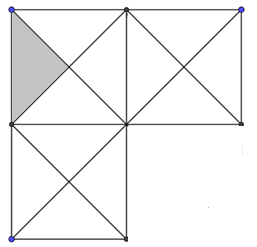
\includegraphics[width=\linewidth]{triangulos6.png}
\caption*{Primeiro tipo}
\end{figure}
\end{minipage}
\begin{minipage}{.2\linewidth}
\begin{figure}[H]
\centering

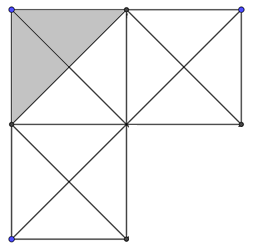
\includegraphics[width=\linewidth]{triangulos7.png}
\caption*{Segundo tipo}
\end{figure}
\end{minipage}
\begin{minipage}{.2\linewidth}
\begin{figure}[H]
\centering

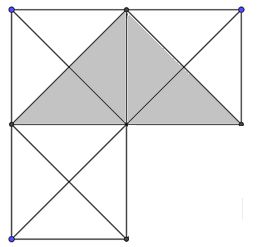
\includegraphics[width=\linewidth]{triangulos8.png}
\caption*{Terceiro tipo}
\end{figure}
\end{minipage}
\begin{minipage}{.2\linewidth}
\begin{figure}[H]
\centering

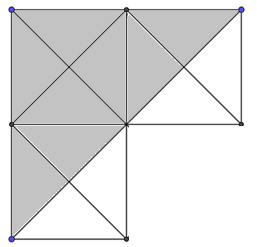
\includegraphics[width=\linewidth]{triangulos9.png}
\caption*{Quarto tipo}
\end{figure}
\end{minipage}
}{1}
\end{answer}

\begin{answer}{Desafios da coloração de mapas}
{
\begin{enumerate}\setcounter{enumi}{1}
\item Escolhido o primeiro triângulo a ser pintado, existem duas possibilidades de cores, a partir dele os outros são pintados de maneira única para atender a restrição. 

\begin{figure}[H]
\centering

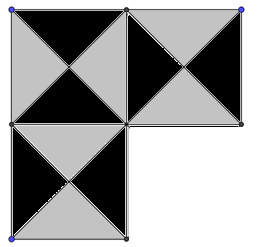
\includegraphics[scale=0.3]{triangulos2.png}
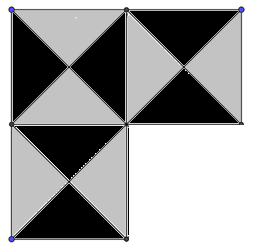
\includegraphics[scale=0.3]{triangulos3.png}
\end{figure}

\item Só existem duas colorações possíveis pois a coloração depende somente da cor escolhida para o primeiro triângulo a ser pintado, esse com duas possibilidades de escolha justificada pelo item b).
\item Seguem algumas possibilidades de resposta para as características:

\begin{enumerate}
\item É possível perceber que a peça é composta por duas figuras coloridas iguais e uma diferente.
\item É possível perceber que a peça é composta por 3 cópias de uma peça menor, sendo que uma delas está rotacionada. 
\item Começando a coloração por um triângulo qualquer, as colorações dos outros triângulos já ficam determinadas.
\item A escolha de que triângulo é colorido primeiro independe pois a coloração obtida será um dos casos detalhados no item \titem{b)}.
\end{enumerate}

\item Utilizando todas as três cores disponíveis para a coloração, seguem algumas possibilidades:
\begin{center}
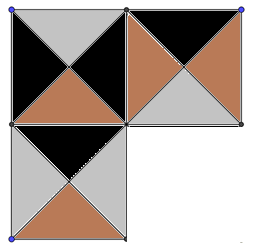
\includegraphics[scale=0.3]{triangulos10.png}
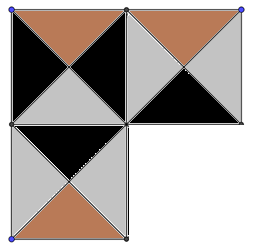
\includegraphics[scale=0.3]{triangulos11.png}
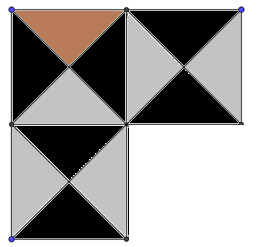
\includegraphics[scale=0.3]{triangulos12.png}
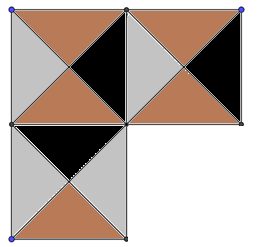
\includegraphics[scale=0.3]{triangulos13.png}
\end{center}

\item Pergunte aos estudantes as estratégias utilizadas por eles e discuta com a turma as estratégias possíveis.

\item É possível que não tenhamos  colorações iguais entre as feitas pelos estudantes na turma. Vejamos porque através da contagem no próximo item. 
\end{enumerate}
}{0}
\end{answer}
\begin{answer}{Desafios da coloração de mapas}
{
\begin{enumerate}[wide]\setcounter{enumi}{7}\small

\item A numeração abaixo ajuda a organizar um caminho para contagem: 
\begin{center}
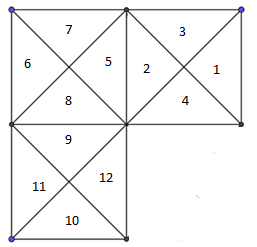
\includegraphics[scale=0.5]{triangulos4.png}  
\end{center}

Olhando para os triângulos de 1 até 4, como existem três cores para pintá-los, dois triângulos terão a mesma cor, por conta da restrição necessariamente será 1 e 2 ou 3 e 4. Imaginando que o triângulo 1 seja igual ao 2, existem $3 \cdot 2\cdot 2 $ maneiras de pintar os triângulos 1,2 3 e 4.  Se o triângulo 1 tiver cor  diferente do triângulo 2 são $3\cdot2 $ possibilidades. Com isso, os quatro primeiros triângulos podem ser pintados de $18 ~~ (3 \cdot 2\cdot 2 +3\cdot2)$ maneiras diferentes. 

O triângulo 5 pode ser pintado de 2 maneiras diferentes, pela restrição fronteiriça com o triângulo 2. Assim, abre-se duas possibilidades, identificar o triângulo 6 com a mesma cor de 5 ou não. Se o triângulo 6 for pintado da mesma cor teremos 2 possibilidades de cor para os triângulos faltantes 7 e 8 totalizando 4 possibilidades, duas se identificarmos os triângulos 7 e 8 com a mesma cor e duas se tiverem cores distintas. Assim, obtemos $2 \cdot 4 = 8$ possibilidades. Já se o triângulo 6 for pintado de cor diferente do 5 com duas possibilidades, os dois triângulos faltantes ficam determinados. Com isso para os triângulos de 6 à 8 são coloridos de $ 12~ ~ (2 \cdot 2 \cdot 2+ 2 \cdot 2)$ maneiras possíveis. 

O raciocínio para os triângulos de 9 à 12 é análogo a coloração dos triângulos de 5 à 8. Como para cada coloração do primeiro existem 12 do segundo e 12 do terceiro, o número total de colorações é dada por: $18 \cdot 12 \cdot 12 = 2592$.


Quanto contamos desta forma, casos de colorações com apenas duas cores são consideradas, mas elas não fazem parte do problema. É possível escolher de 3 maneiras diferentes duas cores para pintar o mapa, e já foi feito no item anterior que com 2 cores existem 2 colorações distintas. Logo foram contados 6 colorações a mais que devem ser retiradas do total. Com isso, o número de maneiras de colorir o mapa inicial com exatamente 3 cores é dada por $2586.$ 

Não seria possível listar todos esses casos, por este motivo os Princípios Fundamentais são usados. 

\item É possível criar mapas que não podem ser coloridos com menos de 4 cores, por exemplo: 
\begin{center} 

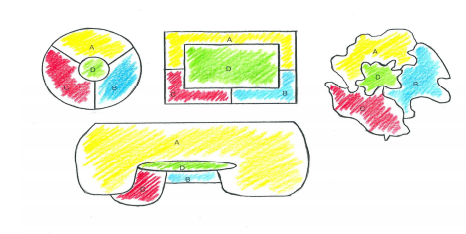
\includegraphics[scale=0.5]{4cores2.png}
\url{https://www.maxwell.vrac.puc-rio.br/22606/22606_3.PDF}
\end{center}

Para que isso ocorra uma região deve ter pelo menos 3 fronteiras e deve estar dentro da região formada pelas outras três ou mais.

\end{enumerate}
}{0}
\end{answer}

\explore{Princípios Fundamentais de Contagem}

Uma gincana está sendo organizada na escola. Para realização das atividades na gincana, a professora de uma turma com 40 estudantes quer organizar os grupos sorteando seus membros. Para isso possui 8 fitas de cada uma das seguintes cores: amarela, vermelha, laranja, branca e preta. Essas fitas serão escolhidas de maneria aleatória sendo misturadas em um recipiente que não seja possível verificar a cor da fita até que seja totalmente retirada.  Joana, uma aluna desta turma, tem um amigo muito querido e está torcendo para que fiquem no mesmo grupo. Será que as chances disso acontecer são grandes ou pequenas?


Para determinar se a chance de um evento ocorrer é grande ou pequena é preciso analisar a taxa de ocorrência deste evento. Em outras palavras, verificar se quantidade de possibilidades do evento ocorrer é grande ou pequena quanto comparada a quantidade total de eventos que podem acontecer. 
Contar o número de casos para responder a dúvida de Joana não é algo que possa ser feito construindo uma lista de todas as possibilidades. Isso levaria muito tempo! Vamos estudar aqui conceitos que ajudam nesta contagem, e em muitas outras, presentes no cotidiano. Esse conhecimento auxilia na tomada de decisões.  

Para caminharmos na direção da solução do problema proposto vamos primeiro desenvolver alguns conceitos de Análise Combinatória. 

\begin{task}{Escolhendo o nome da empresa}

\begin{figure}[H]
\centering

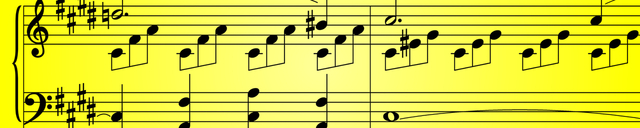
\includegraphics[width=.9\linewidth]{music.jpg}
\end{figure}

Três amigas, Mirella, Rayssa  e Isabela decidiram montar uma sociedade e gostariam que a empresa, do ramo da música, tivesse as inicias (primeira letra) de seus nomes.  

\begin{enumerate}

\item Quais seriam os possíveis nomes para a empresa? 

\item Depois de já terem pensado nas possibilidades de nomes, Letícia decidiu também fazer parte da sociedade. É preciso recomeçar a organização dos nomes ou é possível modificar os nomes já encontrados para que a letra L seja incluída? Quantos seriam agora os possíveis nomes?

\item Se as quatro iniciais tivessem sidos dadas inicialmente a estratégia de contagem teria sido a mesma utilizada no item b)?

\item Quantas seriam as distintas possibilidades usando 5 iniciais diferentes? E 6? E 7? Percebeu alguma regularidade? ( Fazer o caso com 2 letras pode ajudar a pensar na regularidade.)

\end{enumerate}

\end{task}

\begin{knowledge}
$n!$ (lê-se n fatorial) é uma simplificação para a expressão matemática $n!=n \cdot (n-1) \cdot (n-2) \cdots 2 \cdot 1.$ Esse símbolo aparece com muita frequência nos problemas de contagem. Por exemplo, para $n=2,$ $2!= 2 \cdot 1 = 2.$ Tomando agora $n=7,$ $7!=7 \cdot 6 \cdot 5 \cdot 4 \cdot 3\cdots 2 \cdot 1 = 5040.$ Observe que, apesar de $n$ ter crescido pouco, de $2$ para $7,$ o fatorial desses números tem um grande crescimento. A notação de exclamação foi introduzida por Christian Kramp, matemático francês, no trabalho \textit{ Éléments d'arithmétique universelle}. Veja mais em:

\begin{figure}[H]
\centering


\includegraphics[scale=0.3]{frame.png}   
\end{figure}
\end{knowledge}


\begin{task}{Nome da empresa com letras repetidas}


Três amigos, Marcos, Rayssa  e Roberto decidiram montar uma sociedade e gostariam que o nome da empresa, do ramo dos aplicativos, fosse formado pelas inicias (primeira letra) de seus nomes. 

Como seria pensar na quantidade de nomes da empresa se existissem nomes com mesmas iniciais ? Observando as soluções da Atividade \textbf{Escolhendo o nome da empresa} pense nas modificações necessárias para construir a solução deste novo problema.

\begin{enumerate}

    \item Quantos seriam os nomes possíveis se a sociedade tivesse apenas Rayssa e Roberto?
    \item Quantos seriam os possíveis nomes da empresa com os três amigos?
    \item Quantos seriam os nomes  possíveis para a empresa se Letícia decidisse participar da sociedade ?
    \item Quantos seriam os nomes possíveis se a sociedade tivesse quatro pessoas, das quais três possuem nomes com letras iniciais iguais e a outra pessoa letra inicial do nome diferente das demais?
    \item Quantos seriam os nomes possíveis se a sociedade tivesse quatro pessoas, duas a duas com letras iniciais iguais?
\end{enumerate}

\end{task}

\clearpage
\begin{knowledge}
As várias ordenações de letras de uma determinada palavra são chamadas de Anagramas. Seriam como palavas, não necessariamente com sentido, que podem ser formadas a partir de um dado conjunto de letras. Saiba mais sobre a história e curiosidades dos Anagramas em 
\begin{figure}[H]
\centering


\includegraphics[scale=0.3]{frame3.png} 
\end{figure}
\end{knowledge}

\begin{task}{Jogo de dominó}
\textit{Inspirada em \url{ https://olimpiada.ic.unicamp.br/static/extras/obi2019/provas/ProvaOBI2019_f1p1.pdf} }

\begin{figure}[H]
\centering

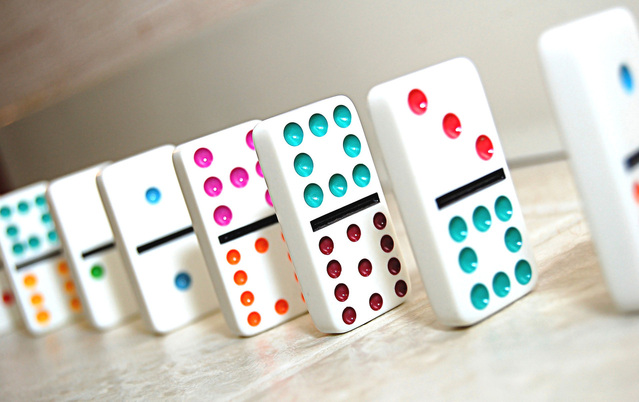
\includegraphics[scale=1]{domino.jpg}
\end{figure}


%{https://pt.freeimages.com/photo/domino-effect-4-1170138}
Em um jogo de dominó cada jogador começa com 7 peças, caso sobrem algumas, estas ficam para serem compradas durante a partida. As peças, todas distintas, são compostas por duas partes, cada uma das partes apresentando pontos que variam de 0 até 6, sendo permitido que a peça tenha duas partes iguais.
 
\begin{enumerate}

\item Escolha um critério de organização das peças de um dominó. Explique aos colegas o motivo dessa escolha.

\item Quantas peças tem um dominó convencional? Qual é o número máximo de jogadores por partida?

\item Imaginando um jogo de dominó com o número de pontos variando de 0 até n em cada parte. Qual o menor número n para que 5 pessoas possam jogar, iniciando com 7 peças cada?

\item Como encontrar o número de peças de um dominó com peças que permitam até 8 pontos em cada um de seus dois lados? 

\item Como saber a quantidade de peças de um dominó que tenha até $n$ pontos em cada um de seus lados?

\end{enumerate}

\end{task}

\begin{knowledge}
Saber se a ordem de organização dos elementos de um agrupamento influencia na contagem é muito importante. Perceba que para o nome da empresa a ordem em que as letras aparecem na palavra muda o nome criado, já para o conjunto de dominós a organização das peças é indiferente para o número total de peças. 
\end{knowledge}

\begin{task}{Desfios da coloração de mapas}
\label{coloracao-mapas}

Alguns desafios de contagem aparecem em redes sociais. O mais atrativo neles é que parecem simples, mas quando percebemos já perdemos horas tentando e não chegamos a solução correta. Quem é que não gosta de um bom desafio, não é?! 
Vejam esse simples mapa abaixo. 

\begin{center}
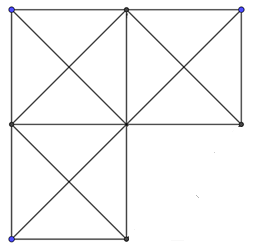
\includegraphics[scale=0.7]{triangulos.png}
\end{center}

\begin{enumerate}
\item Quantos triângulos o mapa possui? Como realizou a contagem?
\item Use duas cores para pintar os triângulos menores de modo que aqueles que tiverem lados em comum não sejam coloridos com a mesma cor. 
\item Compare sua pintura com a do seu colega.  De quantas maneiras distintas foi possível colorir o mapa? 
\item Foi possível perceber alguma característica nas colorações do item b)?
\item Dispondo de três cores, utilize todas para pintar os triângulos menores de modo que aqueles que tiverem lados em comum não sejam coloridos com a mesma cor.
\item Qual foi a estratégia que você utilizou para chegar nessa configuração de cores?
\item Quantas configurações diferentes de cores apareceram na turma?
\item Como podemos contar todas as configurações possíveis?
\item Será que existe um mapa que não possa ser colorido com menos de $4$ cores, seguindo a restrição de que regiões que possuem fronteiras não sejam coloridas coma a mesma cor? Tente encontrar um exemplo. Se ele existe que característica precisa ter? Se não existe, por qual motivo não existe?
\end{enumerate}

\end{task}

\begin{knowledge}
Quatro cores são suficientes para colorir qualquer mapa de modo que regiões fronteiriças (que possuem um lado em comum) não sejam pintadas da mesma cor.  Este problema esta intimamente ligado a Teoria dos Grafos. Saiba mais em:  
%https://teses.usp.br/teses/disponiveis/55/55136/tde-26112016-112047/publico/CarlosLaercioGomesdeLima_revisada.pdf

\begin{figure}[H]
\centering

    
\includegraphics[scale=0.3]{frame (1).png}
\end{figure}


Na Atividade \hyperref[coloracao-mapas]{Desafios da coloração de mapas} você deve ter se perguntado sobre a importância de pensar no número de colorações de um determinado mapa. Esta atividade poderia estar modelando o seguinte problema: Uma escola técnica possui 12 disciplinas e precisa organizar seus horários de exame final tomando o cuidado para que o aluno não tenha que realizar dois exames no mesmo período. As 12 disciplinas poderiam ser associadas aos triângulos pequenos e as fronteiras representariam as disciplinas que possuam alunos em comum para a realização da prova. As provas podem ser organizadas usando apenas dois períodos? Isso pode ser feito de quantas maneiras diferentes? Usando três períodos, quantas são as possibilidades de organização?
Segue também QR Code para o Jogo das Quatro Cores

\begin{figure}[H]
\centering

    
\includegraphics[scale=0.3]{frame4.png}
\end{figure}

%\url{http://www.matematica.seed.pr.gov.br/modules/conteudo/conteudo.php?conteudo=366} 
que consiste em colorir um mapa usando no máximo $4$ cores com as mesmas restrições descritas anteriormente.
\end{knowledge}

\arrange{Princípios Fundamentais de Contagem}

Os problemas estudados em Análise Combinatória são aqueles que se preocupam em contar a quantidade de agrupamentos com determinadas condições. O objetivo é contar todas as variações possíveis sem ter que listar as possibilidades, é quantificar sem necessariamente visualizar. Quando a tarefa é pequena mostrar todos os resultados pode até ser simples e útil, mas no geral as soluções logo se tornam trabalhosas demais. As duas ferramentas descritas aqui resolvem a grande parte dos problemas de contagem.

Para compreender o \textbf{Princípio Multiplicativo} vamos considerar dois questionamentos: De quantas maneiras um grupo pode escolher um(a) capitão(ã) e um(a) vice capitão(ã)? De quantas maneiras um grupo pode escolher dois membros para participar de um jogo de cartas? Vamos considerar aqui o grupo com 8 integrantes que a professora formou lá no início do livro. 

As duas perguntas parecem iguais, mas para o jogo de cartas não faz diferença quem foi o primeiro membro escolhido e quem foi o segundo, importa somente que dois sejam escolhidos. Mas quando se trata de capitão(ã) e vice essa escolha é diferente, pois capitã Júlia e vice Marcos é diferente de capitão Marcos e vice Júlia. 

Para simplificar vamos chamar os membros da equipe de 
$$M_1, M_2, M_3, M_4, M_5, M_6, M_7, M_8.$$

Observe a árvore de possibilidades: 


\begin{figure}[H]
\centering

    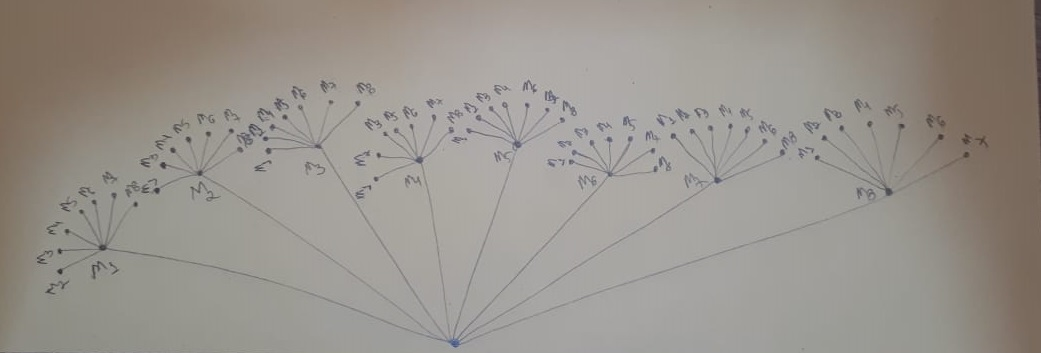
\includegraphics[scale=0.5]{arvore1.jpg}
\end{figure}


Saindo da raiz da árvore existem 8 possibilidades $\{M_1, M_2, M_3, M_4, M_5, M_6, M_7, M_8\}$ para a escolha do primeiro membro. Depois o segundo ramo da árvore, contem as possibilidades que estão disponíveis, após a primeira escolha. Qualquer membro que for escolhido para capitão(ã) tem disponível 7 membros para ser vice, as possibilidades são diferentes, mas as quantidades não. Para encontrar o total podemos somar oito parcelas iguais a 7, cada uma correspondendo a contagem feita tomando como referência um membro da equipe, correspondendo a um ramo da árvore. Este cálculo pode ser simplificado como oito vezes sete :

$$7+7+7+7+7+7+7+7=  8 \cdot 7= 56.$$

De maneira resumida, deve ser realizada a multiplicação do número de possibilidades de escolha do(a) capitão(ã)  pelo número de possibilidades de escolhas do(a) vice. O importante é perceber que nesta contagem $M_1M_2  \neq M_2M_1$, pois nas 8 possibilidades iniciais foram considerados todos os membros, ou seja, tanto $M_1$ quanto $M_2$.  

Ao escolher um representante para ser o(a) capitão(ã), os(as) possíveis vices mudam, mas o número de possibilidades não muda. Por isso o \textbf{Princípio Multiplicativo} pode ser usado, pois se refere a uma soma de parcelas iguais. Mas neste caso como a contagem está sendo feita sempre do mesmo conjunto de dados, a utilização deste princípio leva em conta a ordem dos elementos.

De maneira geral,  se para cada ocorrência de um determinado fato o número de ocorrências de outro fato não se altera, então o número de ocorrências dos dois fatos juntos, ou de maneira sucessiva,  é dado pelo produto das possíveis ocorrências de cada um, é o que garante o \textbf{Princípio Multiplicativo}. 

Este princípio pode ser utilizado em muitos contextos e repetidas vezes. Imagine que a escolha fosse relativa a capitão(ã), vice e um(a) substituto(a). Seriam três posições para serem ocupadas, oito possibilidades para a primeira, sete para a segunda e seis para a terceira. Cada escolha feita para capitão(ã) e vice deixa disponível seis possibilidades de escolha para o(a) substituto(a), logo seriam $8\cdot 7 \cdot 6$ possibilidades de escolha.

Para a construção das duplas na pergunta do jogo de cartas a ordem não é importante, a dupla $M_1M_2 = M_2M_1 = \{M_1,M_{2}\}$. Isso quer dizer que a cada uma das soluções procuradas será contabilizada duas vezes se o \textbf{Princípio Multiplicativo} for utilizado. São duas cópias da mesma solução. por isso a solução procurada é dada por $\dfrac{8 \cdot 7}{2}$.

 Se a ideia fosse escolher trios, da mesma forma seriam $8\cdot 7 \cdot 6$ maneiras de escolher 3 pessoas com ordem de escolha. Pegando uma sequência de três pessoas, digamos $M_1M_2M_3$, elas podem ser organizadas de 6 maneiras diferentes em fila (que corresponde ao número total de trocas de posições dadas entre elas, calculada por 3!=6), mas quando o interesse é por trios, essas seis variações representam o mesmo trio: $M_1M_2M_3=M_1M_3M_2=M_2M_1M_3=M_2M_3M_1=M_3M_1M_2=M_3M_2M_1=\{M_1,M_{2},M_{3}\}.$
 
 Como isso  ocorre para quaisquer três membros diferentes, cada solução procurada foi contabilizada seis vezes, foram contadas seis cópias da mesma solução, e para retirar a repetição é preciso fazer a divisão por $3!=6$, $$\dfrac{8 \cdot 7 \cdot 6}{6} = 8 \cdot 7 = 56.$$

O \textbf{Princípio Multiplicativo} impõe uma ordem quando os elementos são tomados no mesmo conjunto e a divisão deve ser usada quando é preciso retirar a ordem da contagem. Mas se o agrupamento é formado com elementos de conjuntos disjuntos (que não têm elementos em comum) o \textbf{Princípio Multiplicativo} não impõe ordem. Se a ordem for desejada depois de encontrada a solução, deve-se levar em conta as permutações possíveis dos elementos de uma dada solução. 

Para ficar mais claro, considere que será preciso escolher uma dupla de juízes para uma das atividade em sala, sendo um do grupo $G_1=\{G_{11},G_{12},G_{13},$
$G_{14},G_{15},G_{16},G_{17},G_{18}\}$ e um do grupo $G_2=\{G_{21},G_{22},G_{23},
G_{24},G_{25},G_{26},$ $G_{27},G_{28}\}$. Existem 8 possibilidades para a escolha dos membros de cada grupo:


\begin{figure}[H]
\centering


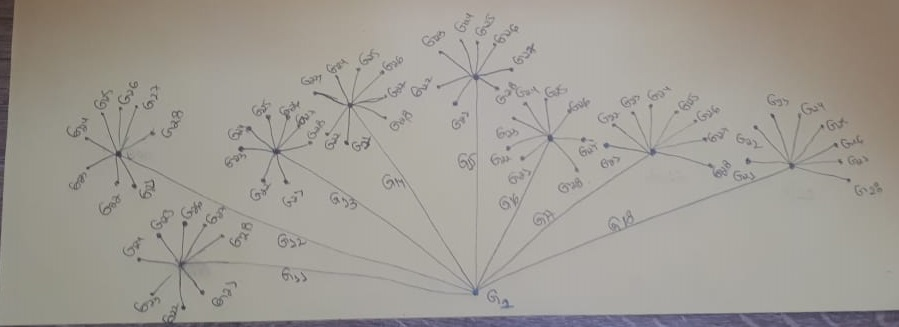
\includegraphics[scale=0.5]{arvore2.jpg}
\caption{$G_{ij}$ indica o membro $j$ do grupo $i$.}
\end{figure}

 $$8+8+8+8+8+8+8+8=  8 \cdot 8.$$
 
Mas neste caso só faz sentido considerar $G_{21}G_{11}$, quando a contagem for organizada a partir do grupo $G_2$, pois $G_{21}$ não faz parte do grupo $G_1$. Para este problema, apesar da escolha estar sendo feita para duplas, não existe a necessidade da divisão por 2, pois não existem cópias da mesma solução. Cada membro foi escolhido de um grupo diferente de possibilidades. Tendo escolhido qualquer membro de $G_1$ restam sempre as mesmas possibilidades para a escolha do membro de $G_2$, que são todos os membros do grupo. Caso seja necessário impor ordem nesta contagem é preciso multiplicar pelas variações possíveis, que seria o mesmo que usar o \textbf{Princípio Aditivo}.

O \textbf{Princípio Aditivo}, diz que se um problema de contagem puder ser separado em problemas menores que não possuam casos em comum, a solução para o problema mais geral pode ser calculada como a soma das soluções dos problemas menores que o compõe. 

Ao dizer que os problemas menores não possuem soluções comuns, a solução geral está sendo construída como soma de soluções que fazem parte de conjuntos disjuntos (conjuntos separados). 

O raciocínio feito para se chegar ao \textbf{Princípio Multiplicativo}  usa do \textbf{Princípio   Aditivo},  pois a solução foi construída como a soma de várias soluções menores. No geral, o \textbf{Princípio Aditivo} aparece em problemas que possuem restrições que devem ser consideradas separadamente. 

Considere que na formação dos juízes duas pessoas não poderiam estar juntas, isso gera restrições na contagem, a solução pode ser dada como a soma de três casos: duplas formadas com  $P_1$ e sem $P_2$; duplas formadas com  $P_2$ e sem $P_1$ e as duplas formadas sem $P_1$ e sem $P_2$. Outra maneira de resolver este mesmo problema é com o uso da subtração. Assim como a divisão é usada para retirar as cópias da solução a subtração é usada para retirar algumas soluções contabilizadas a mais. Neste último problema, a contagem poderia ter sido feita considerando todas as duplas possíveis e depois retirada dela as duplas com $P_1$ e $P_2$ juntas. 
\clearpage
\def\currentcolor{session2}
\begin{objectives}{Jogo da senha}
{
Praticar o uso dos Princípios Aditivo e Multiplicativo em variações dentro do mesmo problema. Elaborar questões de contagem. Diferenciar e praticar problemas que envolvam ordem de elementos. Diferenciar e praticar problemas que envolvam repetição de elementos.
}{1}{1}
\end{objectives}
\mspace{-2.25em}
\begin{sugestions}{Jogo da senha}
{
O esperado para esta atividade é que os estudantes percebam o efeito da ordem e da repetição na contagem. Eles devem ser incentivados a reexplorar o jogo a cada novo questionamento.

\textbf{Tempo de Execução:} A questão pode ser feita em 90 minutos (1 hora e meia) sendo utilizados entre 5 a 10 minutos para os alunos jogarem e experimentarem o jogo,  para o item \titem{a)} até 5  minutos, e para os demais itens entre 5 a 10 minutos cada, lembrando que eles podem voltar ao jogo a cada questionamento feito.
}{1}{1}
\end{sugestions}
\mspace{-1.25em}
\begin{answer}{Jogo da senha}
{
\begin{enumerate}
\item Pode ser organizado na lousa registro do número de tentativas feitas e quantos alunos realizaram cada número. 

\setcounter{enumi}{2}
\item O fundamental é perceber que as cores não podem ser repetidas, uma vez usada uma das seis cores em uma determinada posição ela não poderá ser utilizada novamente. Com isso existem : $6 \cdot 5 \cdot 4 \cdot 3 = 360$ senhas distintas. 
\item Se o jogo não fornecesse nenhuma dica o número máximo de tentativas, sem repetir senhas já feitas, seria o número máximo de senhas possíveis, ou seja, $360$ tentativas.

\item Sendo 6 números ou símbolos seguindo a ideia de serem distintos e não poderem ser repetidos a contagem do número de senhas distintas não mudará, logo $6!$. 

\item Se a repetição de cores é permitida, para cada posição seriam sempre 6 possibilidades, então $6^4=1296.$

\item Seria a soma das senhas começando com números com as senhas começando com cores. Obtemos  $6 \cdot 5 \cdot  10 \cdot 9 $ senhas começando com cores e $10 \cdot 9 \cdot 6 \cdot 5$ senhas começadas em números. Somando teríamos o total de $2 \cdot 2.700= 5.400$ senhas diferentes.
\end{enumerate}
}{1}
\end{answer}
\begin{answer}{Jogo da senha}
{
\begin{enumerate}\setcounter{enumi}{1}
\item É importante destacar que o número apresentado aqui só faz sentido se os estudantes seguirem as indicações dadas pelo jogo para repensar a próxima senha. 
Na primeira tentativa, como são 6 cores possíveis e 4 escolhas, pelo menos duas delas serão acertadas de primeira, mesmo que em lugar errado. Essa dica pode ser dada para os estudantes testarem. No pior caso então, duas cores serão corretas, mas estarão em lugares errados.

\begin{center}
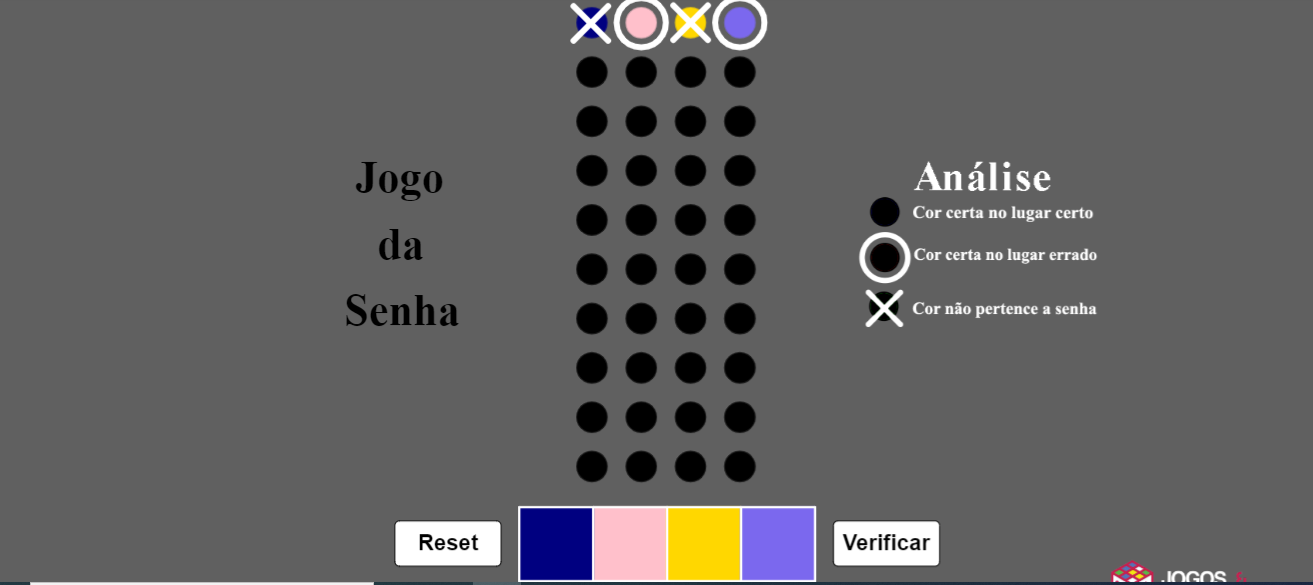
\includegraphics[width=.7\linewidth]{jogosenhaS1.png}
\end{center}
No exemplo dado na figura acima, como as cores azul e amarelo não fazem parte da senha, na segunda jogada já se sabe que as cores envolvidas são vermelho, verde, rosa e lilás. Além disso se sabe que rosa não pode estar na segunda posição e lilás não pode estar na última. No pior dos casos todas as cores estão sempre erradas até a última tentativa. Como cada cor só poderá percorrer 4 espaços de senha, na quarta tentativa a senha terá sido descoberta. 
\end{enumerate}
}{9}
\end{answer}
\clearmargin
\begin{answer}{Jogo da senha}
{
\begin{enumerate}\setcounter{enumi}{7}
\item Uma senha onde a repetição é permitida geraria mais possibilidades de escolha e portanto, maior segurança.

\item Sugestões que levem em consideração o uso de mais símbolos como letras e números que podem se repetir integradas a senha com cores  aumentam o número de possibilidades da mesma.

\item Algumas possibilidades: 1) De quantas maneiras podemos escolher 4 bolas de uma caixa que contenha 6 bolas distintas? 2) De quantas maneiras é possível organizar um grupo com 4 alunos de um total de 6? 3) De quantas maneiras posso pintar 4 brinquedos iguais usando 4 cores de um total de 6?
\end{enumerate}
}{1}
\end{answer}

\practice{Princípios Fundamentais da Contagem}

\begin{task}{Jogo da senha}

\begin{figure}[H]
\centering

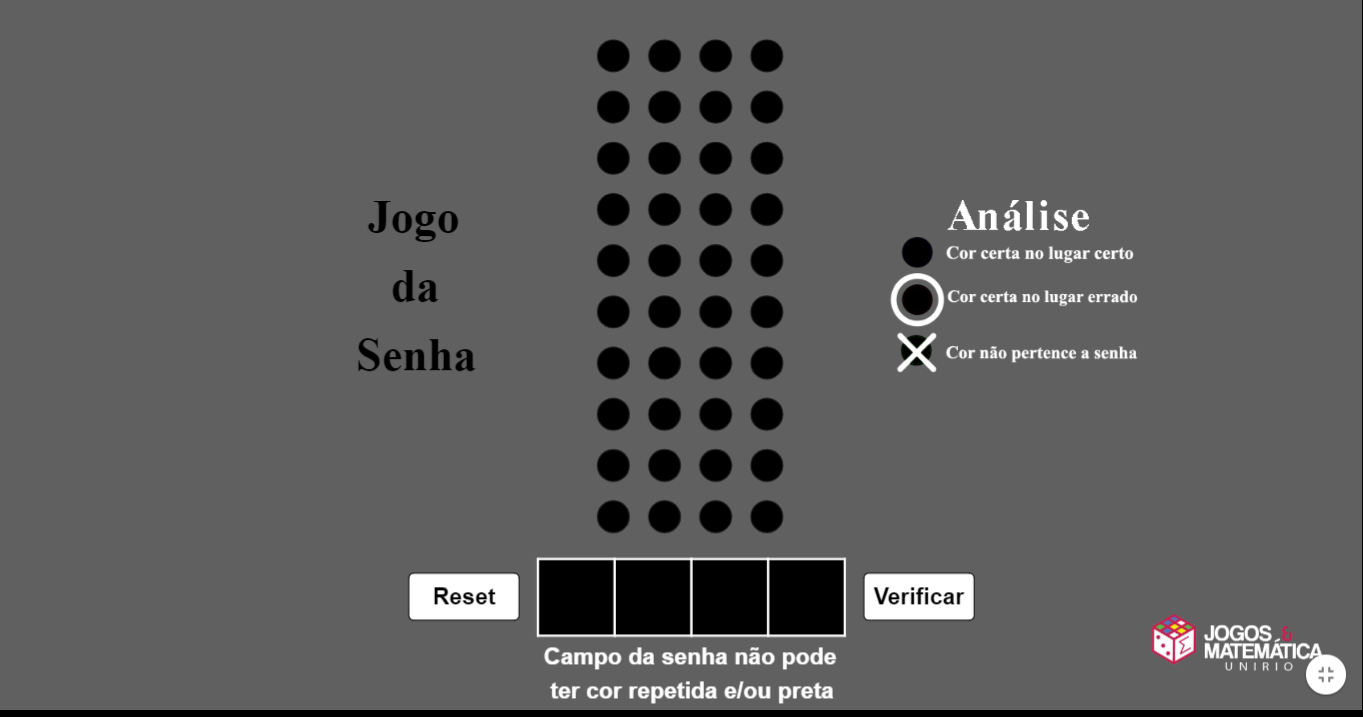
\includegraphics[scale=0.3]{jogosenha.png}
\end{figure}

A senha é composta por 4 cores distintas. Clique em cada um dos 4 quadrados para selecionar uma cor dentre seis disponíveis, e em seguida clique no botão verificar. Sua tentativa será salva nas linhas com 4 bolinhas, e automaticamente é gerado uma análise como pode ser conferida na tela do jogo. O jogador deverá observar análise feita antes de seguir para a próxima tentativa. Vence o jogador que acertar a senha com o menor número de tentativas.



Clique para jogar: \url{https://www.geogebra.org/m/rjyuwp2j}.



Referência: ( Este jogo faz parte de um projeto
\url{https://jogosmatunirio.wordpress.com/jogos-digitais/}) 



Depois de jogar discuta com seus colegas as questões abaixo. 

\begin{enumerate}

\item Qual foi o maior número de tentativas feitas na turma para acertar a senha? 
\item Seguindo todas as dicas, é possível saber qual seria o número máximo de tentativas para acertar a senha? Se sim, determine esse número.
\item Quantas senhas é possível formar neste jogo?
\item Caso o jogo não fornecesse as dicas qual seria o número máximo de tentativas para acertar a senha?
\item Quantas senhas seriam possíveis de ser formadas se as cores fossem trocadas por 6 números ou 6 símbolos sem que seja permitida a repetição?
\item Qual seria o número de senhas possíveis se fosse permitido repetir as cores?
\item Qual seria o número de senhas possíveis se fossem usadas 2 cores distintas e 2 números distintos, de um total de 6 cores e 10 números de modo que as cores fiquem juntas e os números também?
\item Levando em conta que quanto mais possibilidades de senhas mais segurança para os usuários, já que descobrir a senha por tentativas se torna uma tarefa difícil, seria melhor uma senha que permitisse ou não repetição de caracteres?

\item Dada uma senha do tipo dado no exercício, quais modificações poderiam ser feitas em sua construção para tornar mais difícil de determiná-la ?

\item A ordem em que as cores aparecem muda a senha representada. Crie um problema de contagem onde a ordem da escolha não impacta na solução do problema.
\end{enumerate}


\end{task}
\clearpage
\def\currentcolor{session1}
\begin{texto}
{
  \section{Contando Agrupamentos}

A lista de dificuldades apresentada pelos estudantes descritas por \cite{Renan}, inclui não perceberem se os objetos são distintos ou não, e se o problema pressupõe repetição de elementos ou não. Podemos, também, incluir a dificuldade em entender e diferenciar os vários agrupamentos existentes. Deste modo os estudantes sentem dificuldade em diferenciar os tipos de problemas combinatórios. 

Muitas vezes ao tomar contato com uma fórmula os estudantes abandonam o uso do Princípio Multiplicativo apegando-se a diferenciação da ordem na escolha dos objetos. Acabam se perdendo em tentar descobrir qual fórmula usar e travam o raciocínio quando os problemas não são meras aplicações das mesmas. Como aponta \cite{Cristiane} ``É necessário que se tenha a consciência de que o que vai ser   contado influi na forma de contar. Na escola, os alunos podem errar no cálculo relacional por seguirem pistas semânticas.''

A proposta da seção \textbf{Contando Agrupamentos} é trabalhar os diferentes tipos de problemas combinatórios sem necessariamente classificá-los como permutação, arranjo ou combinação. As Atividades apresentam variações que permitem relações com outras Atividades. Os estudantes também serão levados a criarem problemas combinatórios e a analisarem soluções erradas. As tarefas incluem os conceitos com elementos repetidos para que fique claro o impacto dessas modificações no problema, visto que estão presentes em problemas reais.

Os Princípios Aditivo e Multiplicativo foram formalizados na seção anterior, mas serão melhor compreendidos na construção de diferentes agrupamentos.

Outro ponto relevante na questão relativa ao uso das fórmulas é que elas podem esconder a real compreensão dos estudantes sobre o raciocínio combinatório. Por este motivo a avaliação deve ser um instrumento que preza mais pelo raciocínio do que pela aplicações de fórmulas.
}
\end{texto}
\begin{objectives}{Sistema Braille}
{
\begin{itemize}
\item Entender a importância do princípio Aditivo e Multiplicativo nas diversas variações dos problemas de contagem. 
\item Organizar o problema e dividir em casos aplicando diretamente o Princípio Aditivo para a solução.
\end{itemize}
}{1}{1}
\end{objectives}
\clearmargin
\begin{sugestions}{Sistema Braille}
{
O esperado para esta atividade é que os estudantes compreendam e utilizem a  estratégia de contagem  organizando em casos particulares usando, efetivamente, ambos os Princípios Aditivo e Multiplicativo. 

\textbf{Tempo de Execução:} A questão pode ser feita em 30 minutos sendo utilizados até 5  minutos para cada item.
}{1}{2}
\end{sugestions}
\begin{answer}{Sistema Braille}
{
\begin{enumerate}
\item Cada um dos pontos de uma célula Braille pode ou não estar em relevo e, portanto, a cada ponto pode ser associado duas escolhas possíveis. Como temos 6 pontos, pelo Princípio Multiplicativo, o número de possibilidades é igual a $$2 \cdot 2 \cdot 2 \cdot 2 \cdot 2\cdot 2 = 2
^{6}=64.$$ No entanto, não faz sentido ao sistema braille que não  se tenha relevo, e portanto, descartamos essa possibilidade. Logo, o número de diferentes disposições de pontos é dada por $64-1=63.$

\item As células Braille geradas na primeira série são contadas em quatro conjuntos. O primeiro conjunto possui um elemento, símbolo contendo somente o ponto $1.$ O segundo conjunto é determinado por todos os símbolos que possuem o ponto $1$ e são gerados utilizando os pontos $2, 4$ e $5.$
Assim temos os seguintes casos para o segundo conjunto. No primeiro caso o símbolo possui o ponto $1$ e um dos pontos dentre $2,4$ e $5,$ com contagem de $3$ células Braille geradas. Para o segundo caso, o símbolo possui o ponto $1$ e dois pontos dentre $2,4$ e $5.$ Escolhendo dois elementos dentre  $2,4$ e $5$, obtemos $3=\dfrac{3!}{2}$ possibilidades. No terceiro caso, a célula Braille possui os pontos $1,2,4$ e $5,$ e portanto somente uma possibilidade gerada.
O terceiro e quarto conjuntos de células Braille possuem somente um elemento cada, símbolo gerado pelos pontos 2 e 4; e o símbolo gerado pelos pontos $2{,}4$ e 5. Aplicando o Principio Aditivo, obtemos  
$$1+3+3+1+1+1=10$$ 
células Braille geradas na primeira série.\end{enumerate}
}{1}
\end{answer}
\begin{answer}{Sistema Braille}
{
\begin{enumerate}
\setcounter{enumi}{2}

\item O símbolos da sexta série  são contadas em dois conjuntos. O primeiro conjunto possui um elemento, célula Braille contendo somente o ponto $3.$ O segundo conjunto é determinado por todos os símbolos que possuem o ponto $3$ e são gerados utilizando pontos dentre $4, 5$ e $6.$
Assim temos os seguintes casos. No primeiro caso o símbolo possui o ponto $3$ e um dos símbolos dentre $4{,}5$ e $6,$ com contagem de $3$ células Braille geradas. No entanto, a célula constituída dos pontos $3$ e $5$ é elemento da quinta série, logo neste conjunto devemos considerar somente $2$ células Braille.  Para o segundo caso, o símbolo possui o ponto $3$ e dois pontos dentre $4,5$ e $6.$ Escolhendo dois elementos dentre $4,5$ e $6$  , obtemos $3=\dfrac{3!}{2}$ possibilidades. No entanto, a célula constituída dos pontos $3,5$ e $6$ é elemento da quinta série, logo neste conjunto devemos considerar somente $2$ células Braille.  No terceiro caso, a célula Braille possui os pontos $3,4,5$ e $6,$ e portanto somente uma possibilidade gerada. Aplicando o Principio Aditivo, obtemos  
$$1+2+2+1 =6$$ 
células Braille geradas na sexta série.

\item As células Braille determinadas na sétima série são todos os símbolos que podem ser gerados utilizando pontos dentre $4,5$ e $6.$ Assim, temos três casos a serem considerados. O primeiro caso, os símbolos gerados utilizando somente um ponto dentre  $4,5$ e $6,$ nos dando 3 possíveis células Braille. No segundo caso, os símbolos são gerados utilizando dois pontos dentre $4,5$ e $6.$ Escolhendo dois pontos dentre três, obtemos $3=\dfrac{3!}{2}$ possibilidades. No terceiro caso, a célula Braille possui os três pontos  $4,5$ e $6$ e portanto somente uma possibilidade gerada. Aplicando o Principio Aditivo, obtemos  
$$3+3+1 =7$$ 
células Braille geradas na sétima série.

\item Como uma célula braille possui 6 entradas possíveis a um ponto,  possível fazer com 1 ponto 6 células distintas. Com 2 pontos teríamos o total de  obtemos $15=\frac{6 \cdot 5}{2}$ possibilidades, pois escolhemos dois lugares, independente de ordem, dentre seis para serem pontos. Efetuando o mesmo raciocínio, com 3 pontos teríamos o total de $20= \frac{6 \cdot 5 \cdot 4}{3!}$ símbolos possíveis,  com 4 pontos teríamos o total de $15=\frac{6 \cdot 5}{2}$ símbolos possíveis,  com 5 pontos teríamos o total de $6=\frac{6!}{5!}$ símbolos possíveis. Com 6 pontos só temos um símbolo possível que é a completude da célula braille. Somando todas estas possibilidades obtemos 
$$6+15+20+15+6+1=63,$$
resultado obtido no item \titem{a)}. Neste ponto é importante destacar para os estudantes que dois caminhos distintos levaram à mesma solução. 

\item As teclas de um computador possuem muito mais do que $63$ símbolos. Neste caso é importante que a turma pesquise como é possível representar tantos símbolos na simbologia braille. Como ficariam então os números?Alguns números em braille podem ser vistos em elevadores. E a música?            
\end{enumerate}
}{9}
\end{answer}
\clearmargin

% \mspace{-.5em}
\begin{objectives}{Indo de um ponto a outro}
{
\begin{itemize}
\item Entender a importância do Princípio Aditivo e Multiplicativo nas diversas variações dos problemas de contagem. 
\item Organização dos elementos a serem contados através de nomeação e/ou ilustração. Desenvolvimento de lateralidade (direita, esquerda, acima, abaixo, horizontal, vertical).
\end{itemize}
}{1}{1}
\end{objectives}
\mspace{-1.25em}
\begin{sugestions}{Indo de um ponto a outro}
{
Esse exercício pode ser usado não só com o intuito de discutir os Princípios de Contagem, mas como material para a metodologia de levar o estudante ao papel de elaboração de uma questão em contagem. Veja que a situação de deslocamento de um local a outro pode ocorrer em várias situações do cotidiano.

Uma  proposta é por meio da figura. Mostrando a figura aos estudantes, o professor pode indagar sobre situações pelas quais se deslocam de um lugar ao outro. As formulações podem ser pontuadas na lousa e escolhida uma situação e itens de questões do tipo já colocados anteriormente podem ser desenvolvidos.

Seguem duas situações que poderiam ser criadas e reescritas como questões desse tipo: 

\begin{enumerate}[topsep=0pt]
\item Imagine que você está andando pela rua quando recebe uma notificação no celular dizendo que algumas quadras dali pessoas estão conseguindo capturar o Pikachu, um dos Pokémons mais famosos. No entanto, você precisa chegar até o local de forma rápida e precisa, pois o monstrinho virtual pode simplesmente sumir do aplicativo. Com um mapa, observa que está no ponto $A$ e precisa chegar ao ponto $B.$

\item Observe a figura e imagine que a sua escola fique no ponto $B$. Um colega de sala mora no ponto $A$ e esqueceu seu aparelho celular na escola. Você o encontrou e deseja devolver, poderá levar o celular até casa dele, tendo em vista que entende o desespero de quem perde o celular. O problema é que você não tem a menor ideia de qual caminho ele costuma fazer para ir até a escola.
\end{enumerate}

Outra observação é entender que o estudante pode achar que faz sentindo tomar um caminho de $A$ até $B$ voltando quarteirões e andando nas outras direções propostas como esquerda e abaixo. Assim, essa restrição deve ficar clara na explicação e formulação do exercício para essa proposta.

\textbf{Tempo de Execução:} A questão pode ser feita em 25 minutos sendo utilizados até 5  minutos para cada item. A proposta pode ter tempo de execução maior caso queira adicionar uma metodologia proposta nas Observações e Recomendações, nesse exercício.
}{0}{0}
\end{sugestions}
\begin{answer}{Indo de um ponto a outro}
{
\begin{enumerate}
\item Para traçar um caminho  os alunos podem  utilizar do desenho e escolher um caminho com lápis colorido. Ou ainda, podem nomear com números ou letras cada segmento vertical e horizontal montando uma sequência que entre os pontos $A$ e $B.$
%aqui eu queria um desenho feita a mão com lápis, o que acha? 
%Boa ideia.

\item Questão feita pela turma. Esperamos que vários caminhos sejam observados.

\item Questão feita pela turma. Para essa questão é esperado que o aluno descreva o caminho de $A$ até $B$ utilizando conceitos como : direita, acima, horizontal e vertical. 


\item Se a restrição é usar somente as direções direita e para cima de forma a sair de $A$ e chegar em $B,$ os caminhos devem ter os mesmo comprimentos totalizando $7$ quarteirões. 

\item Para sair do ponto $A$ e chegar ao ponto $B$ são necessários andar $3$ quarteirões para direita (ou horizontais) e $4$ para cima (ou verticais). Totalizando $7$ quarteirões. Podemos contar então o número de maneiras de se permutar $HHHVVVV$, que são $7$ elementos, mas $3$ de um determinado tipo e $4$ de outro, para retirar as contagens feitas de trocas entre os $H's$ e entre os $V's$ é preciso dividir por  que é dado por $4!\cdot3!$ $$\dfrac{7!}{4!\cdot3!}.$$  Outra maneira de se pensar que o caminho é feito de sete escolhas, em quais  $3$ serão feitos movimentos horizontais, usando o princípio multiplicativo e o fato da ordem de escolha dos momentos não ser importante, importa apenas quais os momentos escolhidos, a solução pode ser pensada como:
$\dfrac{7 \cdot 6 \cdot 5}{3!}.$
\end{enumerate}
}{1}
\end{answer}

\begin{objectives}{Jogo da Mega-Sena}
{
Relacionar o uso de contagem para compreensão de fatos da realidade;
}{1}{2}
\end{objectives}
\mspace{-2.25em}
\begin{sugestions}{Jogo da Mega-Sena}
{
Para realizar esta atividade não é necessário nenhum conhecimento profundo de probabilidade, apenas compreender que representa as chances de um evento acontecer e pode ser calculado diretamente pelo quociente do número de possibilidades de ocorrer o evento sobre o número de casos possíveis.  Não temos aqui o objetivo de ensinar o conteúdo de Probabilidade, mas podemos sim relacioná-lo a atividades de contagem. Se sentir que deve melhorar essa explicação, pode utilizar conteúdo do livro texto de Probabilidade e atividades introdutórias do conteúdo.
}{1}{2}
\end{sugestions}
\begin{answer}{Jogo da Mega-Sena}
{
\begin{enumerate}
\item São 6 dezenas sorteadas, isso pode ser feito de 
\small
$$\dfrac{60 \cdot 59\cdot 58 \cdot 57 \cdot 56 \cdot 55}{6!}= 50.063.860$$
\normalsize
maneiras diferentes. A a ordem em que as dezenas foram sorteadas não impactam no resultado final, por este motivo a divisão por $6!$ foi realizada. Quem ganha acerta uma dessas possibilidades, e portanto temos a probabilidade 
\small
$$\dfrac{1}{\left[\dfrac{60 \cdot 59\cdot 58 \cdot 57 \cdot 56 \cdot 55}{6!}\right]} = \dfrac{1}{50063860}$$
\normalsize
de ganhar o prêmio da Sena.

Para acertar a Quina é preciso acertar 5 dos números sorteados e errar o outro. Para acertar cinco  números  existem $\dfrac{6\cdot 5 \cdot 4 \cdot 3 \cdot 2}{5!}$ maneiras e para errar o outro existem $54$ possibilidades, dentre 6 sorteados. Pelo Princípio Multiplicativo, no total então será $\dfrac{6 \cdot 5 \cdot 4 \cdot 3 \cdot 2 \cdot 54}{5!} = 324.$ São $324$ possibilidades de acertar. Assim, as chances de obter uma quina pode ser vista como o quociente $\dfrac{324}{50063860}$ O que corresponderia a aproximadamente 1 em $154.518$. Do mesmo modo para acertar a Quadra é preciso acertar quatro e errar dois. Isso pode ser feito de $\dfrac{6 \cdot 5 \cdot \cdot 4 \cdot 3 \cdot 2}{4!}\cdot \dfrac{54\cdot53}{2!}=21465 maneiras.$ O que representa 1 em $2332.$
\end{enumerate}
}{1}
\end{answer}
\begin{answer}{Jogo da Mega-Sena}
{
\begin{enumerate}\setcounter{enumi}{1}

\item Quando sete dezenas são escolhidas em um jogo com seis números existem  $\dfrac{7 \cdot 6 \cdot 5 \cdot 4 \cdot 3 \cdot 2}{6!}=7$ possibilidades de acertar o jogo. Por este motivo é preciso pagar por 7 jogos. Que corresponde a $R\$ 31,50.$

\item Pelo item \titem{b)}, para o jogo da Sena, basta multiplicar as chances de escolha de seis números por 7. No caso da Quina com 7 números, para acertar cinco números e errar um dentre os 6 sorteados  existem  $\dfrac{7\cdot 6 \cdot 5 \cdot 4\cdot 3}{5!}\cdot 53$ possibilidades. Assim, as chances de obter uma quina pode ser vista como o quociente $\frac{1113}{50063860},$ ou aproximadamente $\dfrac{1}{44981}.$ 
No caso Quadra temos $\dfrac{7 \cdot 6 \cdot 5 \cdot 4}{4!}\cdot \dfrac{53\cdot 52}{2}$ de acertar 4 números e errar dois dentre os $6$ sorteados, o que equivale a probabilidade $\dfrac{1}{1038}.$

\item Como os números são equiprováveis, ou ainda, tem a mesma chance de serem escolhidos, para a Sena, fazer sete jogos de 6 números é igual a fazer um jogo de 7 números,  uma vez que ambos casos seriam 7 chances de ganhar o prêmio (itens b) e c)). No entanto, no caso da Quina, um jogo com 7 números tem-se $\dfrac{1}{44981}$  chances de ganhar quanto jogar $7$ jogos na Quina equivaleria a $\dfrac{7}{154.518},$  aproximadamente $\dfrac{1}{22074}.$  Se fizermos $7$ jogos de $6$ números, nossa probabilidade se multiplica em $7,$ logo é maior as chances de ganhar na Quina fazendo $7$ jogos de $6$ números.  Analogamente, para a Quadra, um jogo com 7 números tem-se $\dfrac{1}{1038}$ chances de ganhar em relação a um jogo de $6$ números. Se fizermos $7$ jogos de $6$ números, nossa probabilidade se multiplica em $7,$ logo fica 7 em $2332,$ aproximadamente a $\dfrac{1}{333},$ logo  é maior as chances de ganhar na Quadra fazendo $7$ jogos de $6$ números. 

\item Para fazer o jogo com 6 números pago $R\$4,50.$ Temos $50.063.860$ possibilidades de jogos possíveis, então iria ter que dispor de $R\$ 225.287.370$ milhões de reais. Como o prêmio de $R\$ 6$ milhões, sem descontar os impostos, é menor que o valor gasto para fazer todas as apostas possíveis, não valeria a pena jogar todos as combinações. Ganhando sozinho, somente valeria a pena fazer todos os jogos se o prêmio fosse maior do que o valor empregado de  $R\$ 225.287.370$ milhões de reais. 
\end{enumerate}
}{0}
\end{answer}
\begin{objectives}{Alocando-se no cinema}
{
\begin{itemize}
\item Entender a importância do princípio Aditivo e Multiplicativo nas diversas variações dos problemas de contagem. 
\item Compreender que a tomada de decisão leva a caminhos de contagem distintos, e que começar por restrições facilita a resolução do problema. 
\end{itemize}
}{1}{1}
\end{objectives}
\mspace{-2.25em}
\begin{sugestions}{Alocando-se no cinema}
{
O esperado para esta atividade é que os estudantes percebam que não existe caminho único para organização das soluções, mas que é preciso primeiro organizar as restrições do problema. Assim, tomar decisões distintas leva a  caminhos de contagem distintos. Também é esperado que o aluno entenda que deve ser tomadas as restrições primeiramente na tomada de decisão pois isso facilita a contagem.

\textbf{Tempo de Execução:} A questão pode ser feita em 20 minutos sendo utilizados até 5 minutos para cada item. 
}{1}{1}
\end{sugestions}
\begin{answer}{Alocando-se no cinema}
{
\begin{enumerate}
\item Cada grupo terá uma opinião diferente sobre a estratégia. Em termos de contagem tomar os  pontos de restrições mais difíceis facilita a contagem (quem não gostava de determinado lugar).

\item Existem outras maneiras, a ideia é começar sempre pelas restrições. Poderia ser: $B_1$: Alocar quem não gosta de sentar na frente no fundo, depois $B_2$ alocar quem não gosta do fundo na frente e, por último, os que não apresentam exigências $B_3$.  

Outra possibilidade seria $C_1$ : começar alocando nas poltronas da frente os que não gostam de se sentar no fundo, depois $C_2$ alocando no fundo os que não gostam da frente e por último $C_3$ os que não possuem restrições. Outra possibilidade seria alocar os que possuem restrições com o fundo na frente, depois completar as poltronas da frente com os que não apresentam restrições, depois colocar os que não gostam de sentar na frente no fundo e só por último alocar os que não possuem restrições. 

\item Começando a organização pelos que são indiferentes alguns cuidados precisam ser tomados, é preciso que fiquem disponíveis lugares que atendam as restrições. No fundo poderia escolher um lugar para colocar um amigo que não tem preferência, deixando três lugares para os que precisam ir para o fundo, depois alocando os que não tem preferência na frente, automaticamente sobrará o espaço para os que não podem sentar no fundo. 
\item A ideia é que percebam que para contar é necessário transformar as ações anteriormente pensadas em operações matemáticas. 

$A_1:$ Alocou os 3 que não gostam de sentar-se na frente, nas poltronas do fundo: Para o primeiro existem 4 possibilidades de poltrona, para o segundo 3 e para o terceiro 2, pelo princípio multiplicativo : $4\cdot 3 \cdot 2= 24$;

$A_2:$ Colocou no lugar que sobrou na parte de trás uma amigo que é indiferente ao lugar: São sete amigos que não possuem restrições, qualquer um pode sentar-se ali. São então 7 maneiras de realizar esta ação;

$A_3:$ Na frente colocou os outros amigos que faltavam: Sobraram 8 amigos para ocupar 8 lugares, isso pode ser feito de $8!$ maneiras. Como para cada maneira distinta de realizar a $A_1$ existem 7 maneiras de organizar a $A_2$ e $8!$ maneiras de organizar a $A_3$, o Princípio multiplicativo deve ser usado:
$$24 \cdot 7 \cdot 8!= 6.773.760$$
maneiras distintas de organizar os amigos nas poltronas do cinema. 
Utilizando a notação dada no item \titem{b)},\small
\begin{align*}
B_1&: 4\cdot 3 \cdot 2 \\
B_2&: 8 \cdot 7\\
B_3&: 7!
\end{align*}
Pelo Princípio Multiplicativo: 
$$24\cdot 56 \cdot 7!= 6.773.760.$$ 
E
\begin{align*}
C_1&: 8 \cdot 7\\
C_2&: 4\cdot 3 \cdot 2 \\
C_3&: 7!.
\end{align*}
Pelo Princípio Multiplicativo: 
$$ 56 \cdot 24 \cdot 7!= 6.773.760.$$
\end{enumerate}
}{9}
\end{answer}
\begin{objectives}{Analisando a solução do colega}
{
\begin{itemize}
\item Entender a importância do princípio Aditivo e Multiplicativo nas diversas variações dos problemas de contagem.
\item Diferenciar e praticar problemas que envolvam ordem de elementos. 
\item Diferenciar e praticar problemas que envolvam repetição de elementos. 
\item Analisar resoluções. 
\end{itemize}
}{1}{1}
\end{objectives}
\mspace{-2.25em}
\begin{sugestions}{Analisando a solução do colega}
{
O esperado para esta atividade é que os estudantes percebam que algumas estratégias de contagem contam possibilidades a menos ou a mais e saibam analisar criticamente uma solução apresentando os erros e sugerindo correções. É importante nesse ponto o aluno reconhecer alguns distratores na  interpretação de problemas envolvendo repetição e ordem de elementos distintos.

\textbf{Tempo de Execução:} A questão pode ser feita em 30 minutos sendo utilizados de 5  a 10 minutos para cada item. 
}{1}{2}
\end{sugestions}
\begin{answer}{Analisando a solução do colega}
{
\begin{enumerate}
\item O erro está no raciocínio tomado no ponto \titem{2.} o Princípio Multiplicativo deve ser usado na contagem do número de escolha das mulheres, separadamente no número de escolha dos homens e depois multiplicado. Pois estes são conjuntos distintos. A solução correta seria:
                    
$$\dfrac{22\cdot 21}{2!} \cdot \dfrac{ 18 \cdot 17 \cdot 16 \cdot 15}{4!}=706.860.$$
\item
\begin{enumerate}[label=\titem{\arabic*.}]
\item O grupo não considerou que é preciso ter pelo menos dois homens, neste caso as soluções seriam, duas mulheres e quatro homens, três mulheres e três homens e quatro mulheres e dois homens. As três possibilidades podem ser calculadas separadamente e somadas.  
\setcounter{enumii}{2}
\item Não é possível juntar todas as pessoas para completar as vagas restantes, isso geraria soluções repetidas. Exemplo: Escolho primeiro Maria e Bruna, quando conto a segunda parte, suponha que escolha Joice e Marta. Mas estou contando também, inicialmente Marta e Bruna, depois Maria e Joice. Ou seja, este mesmo grupo foi contado mais de uma vez na solução apresentada. 
\end{enumerate}
A solução correta seria:\small
$$\dfrac{22\cdot21 }{2!}\cdot \dfrac{18 \cdot 17 \cdot 16 \cdot 15}{4!}+\dfrac{22\cdot21\cdot 20 }{3!}\cdot \dfrac{18 \cdot 17\cdot 16}{3!}+\dfrac{22\cdot21\cdot 20 \cdot 19 }{4!}\cdot \dfrac{18 \cdot 17}{2!},$$
igual a $3.082.816.$
\end{enumerate}
}{1}
\end{answer}
\clearmargin

\mspace{.5em}
\begin{answer}{Analisando a solução do colega}
{
\begin{enumerate}\setcounter{enumi}{2}
\item O raciocínio tomado em \titem{1.} está correto, já tendo o total é possível retirar os casos que não se quer. Mas o grupo usou o resultado do item anterior que estava errado e ainda repetiu um raciocínio errado que é de juntar todas pessoas para a escolha de 4. 

Solução correta, contar todas as comissões com Eduardo e Lucas: Seriam as comissões só com os dois e quatro mulheres; os dois mais um homem e três mulheres; os dois mais dois homens e 2 mulheres. Assim, temos
$\dfrac{22 \cdot 21 \cdot 20\cdot 19}{4!}+16 \cdot \dfrac{22 \cdot 21 \cdot 20}{3!}+\dfrac{16 \cdot 15}{2!}\cdot \dfrac{22 \cdot 21}{2!} = 84.295$ comissões com Eduardo e Lucas, número esse que deve ser retirado do total indicado no item \titem{b)}.
\end{enumerate}
}{1}
\end{answer}
\begin{objectives}{Produzindo Acessórios}
{
Entender a importância do princípio Aditivo e Multiplicativo nas diversas variações dos problemas de contagem. Aplicar os Princípios Aditivo e Multiplicativo para problemas em contagem de objetos simétricos e com repetição.
}{1}{1}
\end{objectives}
% \mspace{-2.25em}

\begin{sugestions}{Produzindo Acessórios}
{
Primeiramente, por ser um exercício que envolve construção de acessórios que podem não ser comuns ao estudante, o professor deve se atentar a interpretação dos objetos em questão. O esperado para esta atividade é que os estudantes percebam a mudanças de contagens com objetos simétricos e como se dá uma problema de escolha de objetos que podem ser repetidos (combinação completa e permutação com repetição).

\textbf{Tempo de Execução:} A questão pode ser feita em 70 (1 hora e 10) minutos sendo utilizados de 5 a 10 minutos para cada item.
}{1}{1}
\end{sugestions}

\explore{Contando Agrupamentos}

O número de maneiras de se retirar 3 bolas amarelas e 2 vermelhas de uma urna com 5 bolas, sem reposição, tem alguma relação com o número de maneiras de se escolher 3 pessoas de um grupo de 5? Será que problemas completamente diferentes podem ter a mesma solução?

\begin{task}{Sistema Braille}

\textit{Esta atividade está baseada no texto: 
 \url{http://www.ibc.gov.br/images/conteudo/DPPE/Geral_departamento/2019/colecaoapostilas/Simbologia-Braille_2019_public.pdf} Todas as imagens forma retiradas desta bibliografia.}
 
 
 A atividade foi pensada para ser relacionada o material de Pensamento Computacional.
 
 
 
 Criado por Louis Braille, braille é um sistema de escrita e leitura tátil. Ele é determinado por um arranjo de seis pontos em relevo, dispostos em três linhas, com dois pontos em cada linha. O conjunto desses seis pontos é também conhecido como \textit{cela braille} ou \textit{célula braille}, com ilustração dada por  

\begin{figure}[H]
\centering

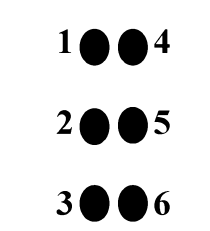
\includegraphics[scale=0.4]{braille2.png}
\end{figure}

Os pontos da célula braille são numerados na seguinte forma:

\begin{itemize}
    \item coluna da esquerda (do alto para baixo) pontos 1, 2 e 3;
    \item coluna da direita (do alto para baixo) pontos 4, 5 e 6.
\end{itemize}
A ordem Braille é uma organização dos símbolos em 7 séries.
\begin{itemize}
    \item A primeira série é denominada série superior constituída pelo símbolo contendo somente o ponto 1; por todos os símbolos que possuem o ponto 1 e são gerados utilizando pontos dentre 2, 4 e 5; o símbolo gerado pelos pontos 2 e 4; e o símbolo gerado pelos pontos 2, 4 e 5.
    \item A segunda série é construída acrescentando o ponto 3 a cada símbolo da primeira série;
    \item A terceira série resulta da adição dos pontos 3 e 6 a cada símbolo da primeira série;
    \item A quarta série é construída com a inclusão do ponto 6 a cada símbolo da primeira série;
    \item A quinta série é denominada série inferior constituída pelo símbolo contendo somente o ponto 2; por todos os símbolos que possuem o ponto 2 e são gerados utilizando pontos dentre 3, 5 e 6; o símbolo gerado pelos pontos 3 e 5; e o símbolo gerado pelos pontos 3,5 e 6.
    \item A sexta série possui como elementos a célula Braille contendo somente o ponto 3; os símbolos contendo o ponto 3 e gerados utilizando pontos dentre 4, 5 e 6; não contados anteriormente na quinta série.
    \item A sétima série é formada pelas sinais gerados somente pelos pontos da coluna direita, ou ainda, todas as células geradas utilizando pontos dentre 4, 5 e $6.$
    
\end{itemize}

\begin{figure}[H]
\centering

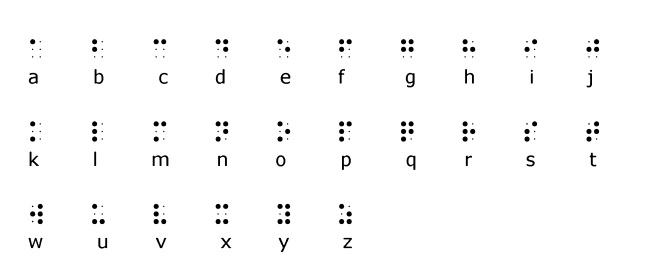
\includegraphics[scale=0.5]{alfabeto.jpg}
\caption{Alfabeto Braille}
\end{figure}

 
 
 \begin{enumerate}
     \item As diferentes disposições dos pontos na célula Braille permitem a formação de quantos símbolos braille?
     \item Quantos elementos possui a primeira série?
     \item Quantos elementos possui a sexta série?
     \item Quantos elementos possui a sétima série?
     \item Quantos símbolos é possível fazer com 1 ponto? Com 2 pontos? Com 3 pontos? Com 4 pontos? Com 5 pontos? Com 6 pontos? Somando todas estas possibilidades qual o valor encontrado?
      \item Olhando, por exemplo, para o teclado de um computador é possível representar todas as teclas por algum símbolo descrito no item a)? 
     
 \end{enumerate}

\end{task}

\begin{knowledge}
A técnica empregada no item \titem{d)} desta atividade, fazer a contagem por dois caminhos distintos e com isso concluir que expressões são iguais, é chamada de demonstração combinatória e é muito utilizada na matemática discreta. Algumas demonstrações que levariam muito tempo para serem feitas algebricamente são demostradas rapidamente por argumentos combinatórios. Veja o vídeo \textit{ PAPMEM - Janeiro de 2020 - Como mexer com coeficientes binomiais sem sujar as mãos}: \url{https://www.youtube.com/watch?v=69HLi6kG_us} para conhecer algumas demonstrações.
\end{knowledge}

\begin{task}{Indo de um ponto a outro}

Com um mapa abaixo, suponha que você está no ponto $A$ e precise chegar ao ponto $B.$ 

\begin{figure}[H]
\centering

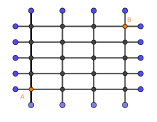
\includegraphics[scale=1.3]{caca_tesouro.png}
\end{figure}

\begin{enumerate}
\item Trace um possível caminho de $A$ até $B$ sendo possível somente andar nas  direções direita e para cima.
\item Compare os caminhos com os do colega de grupo, depois da turma. Tiveram muitos caminhos distintos?
\item Escolha um dos caminhos e dê instruções para um outro amigo da turma, explicando como chegar. 
\item Se todos os quarteirões têm a mesma medida, os caminhos da turma tiveram comprimentos iguais ou diferentes?
\item Seguindo as restrições do problema, qual o número de diferentes caminhos existentes entre você e o ponto $B?$ 

\end{enumerate} 

\end{task}
\clearpage

\begin{task}{Jogo da Mega-Sena}
Passando pelo site do Banco Caixa Econômica Federal é possível encontrar a seguinte tabela de probabilidades. A probabilidade aqui está definida como uma taxa, que representa a chance de ganhar o prêmio, calculada como a divisão entre o número de casos favoráveis e o total de possibilidades de sorteios do prêmio.  
  

\begin{figure}[H]
\centering

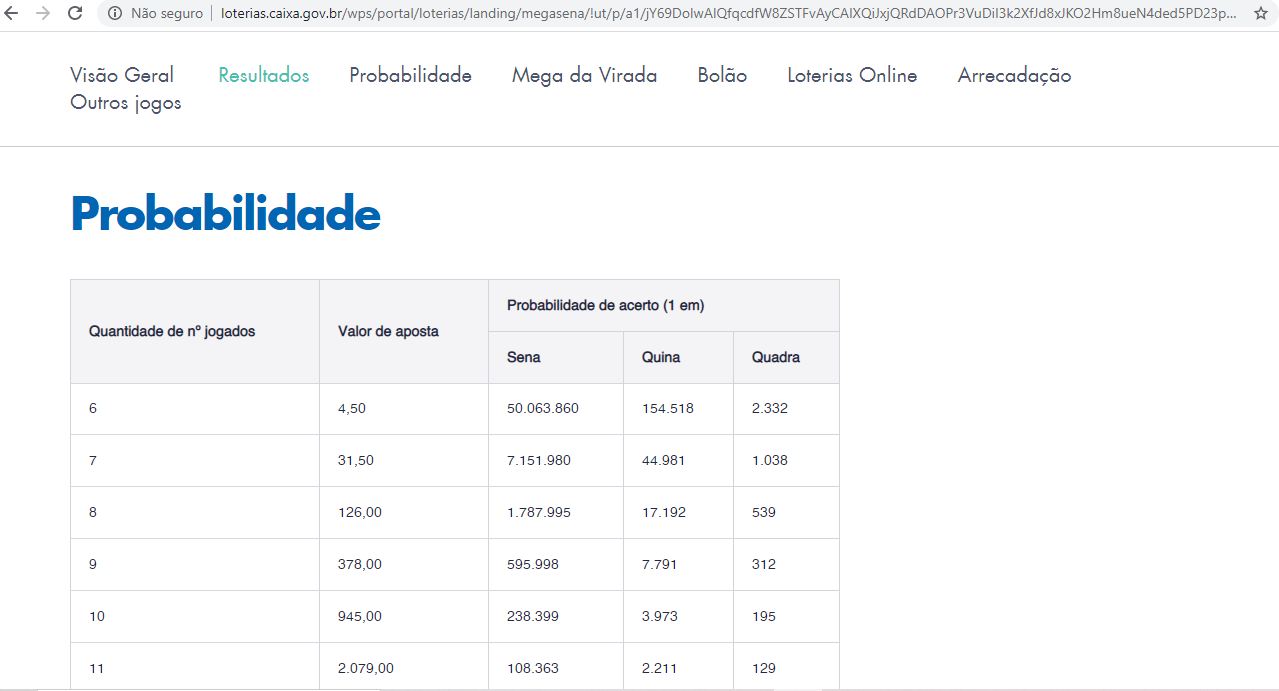
\includegraphics[width=.9\linewidth]{caixa_c.png}
\end{figure}


Sabendo que o jogo é feito com a escolha de pelo menos 6 números dentre as possibilidades de 1 até 60. Responda:

 \begin{enumerate}
     \item Como calcular a probabilidade de ganhar o prêmio da Sena ( acertar os seis números), Quina (acertar 5 números) e Quadra (acertar 4 números) com um jogo de 6 números?
     \item Para fazer o jogo com 6 números pago $R\$4,50$. Por qual motivo a escolha de sete números me custa  $R\$31,50$?
     \item E como recalcular as probabilidades para os prêmio da Sena, Quina e Quadra com 7 números?
     \item Fazendo 7 jogos de 6 números tenho maior probabilidade de ganhar do que fazendo 1 jogo de 7 números?
     \item A estimativa de prêmio do próximo jogo da Sena é de $R\$ 6$ milhões. Para fazer o jogo com 6 números pago $R\$4,50,$ quanto eu tenho que dispor de dinheiro para jogar todas as possibilidades do sorteio ? Valeria a pena jogar todos as combinações possíveis? Senão, supondo que somente pudesse ganhar sozinho, quanto deveria ser o prêmio para que valesse a pena fazer todas as apostas possíveis para a Sena ?
\end{enumerate}
\end{task}
\clearpage

\begin{task}{Alocando-se no cinema}
Um grupo de 12 amigos chegaram bem tarde para assistir um filme no cinema, não sendo possível encontrar todos os lugares juntos. Havia 8 lugares na parte da frente e 4 lugares na parte de trás da sala de cinema. Levando em conta que 2 deles não gostam da ideia de sentar-se no fundo e 3 deles não gostam da ideia de sentar-se na frente. Gabrielly decidiu então organizar a galera, visto que não foi permitido que se sentassem no corredor. Certeza que optariam por esse caminho! Observe a sequência de decisões (ações) que ela tomou:

\begin{itemize}
\item $A_1:$ Alocou os 3 que não gostam de 
sentar-se na frente, nas poltronas do fundo;

\item $A_2:$ Colocou no lugar que sobrou na parte de trás uma amigo que é indiferente ao lugar;

\item $A_3:$ Na frente colocou os outros amigos que faltavam. 
\end{itemize}


\begin{enumerate}
\item Acredita que a estratégia de organização foi eficaz? Por quê?
\item Existe outra maneira de organizar os amigos sem ferir as preferências?
\item Seria possível começar a organizar os amigos por aqueles que são indiferentes ao lugar? 
\item Pedro não gostou da organização pensada, mas diante das inúmeras possibilidades de organização do grupo desistiu de tentar. São mesmo muitas maneiras distintas de organização se as poltronas são numeradas? Como fazer para contar todas?
\end{enumerate}
\end{task}

\begin{task}{Analisando a solução do colega}
O seguinte exercício foi apresentado pela professora para uma turma que estava estudando Análise Combinatória. Por ter várias restrições, as soluções foram bem variadas. A proposta agora é analisar uma solução apontando os erros e acertos no raciocínio do grupo. Para os erros é necessário apontar um possível caminho para correção. Como o seu grupo resolveria este mesmo problema?
 

 Observe a notícia que trata da representatividade feminina nas eleições e responda as questões propostas a seguir:
 

 
"De acordo com o secretário Judiciário do Tribunal Superior Eleitoral (TSE), Fernando Alencastro, a partir de 2020, as legendas deverão encaminhar à Justiça Eleitoral, juntamente com o Demonstrativo de Regularidade de Atos Partidários (DRAP), a lista de candidatas que concorrerão no pleito, respeitando-se o percentual mínimo de 30\% e o máximo de 70\% para candidaturas de cada sexo. A regra está prevista no artigo 10, parágrafo 3º da Lei nº 9.504/1997 (Lei das Eleições)."


\begin{figure}[H]
\centering

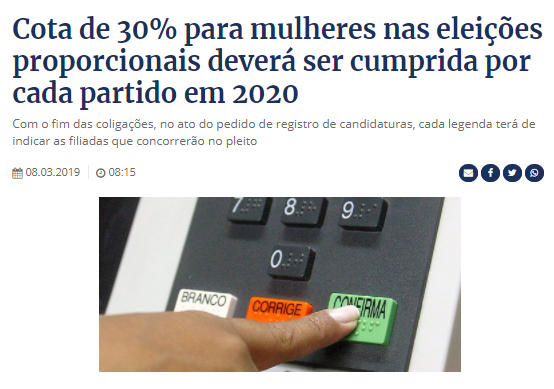
\includegraphics[width=.75\linewidth]{cotafe.png}

\end{figure}


Pensando na importância da representatividade feminina para além das questões políticas e considerando uma turma de 22 estudantes mulheres e 18 estudantes homens responda os questionamentos abaixo. 
 
\begin{enumerate}
\item Quantas comissões de 6 estudantes é possível formar, mantendo exatamente o mínimo de representação feminina?

\textit{Solução do grupo:}  

\begin{enumerate}[label=\titem{\arabic*.}]
\item Para manter exatamente o mínimo de representação feminina a equipe deve ter exatamente 2 mulheres.
\item Usando o princípio multiplicativo e considerando o número de mulheres e homens; e depois levando em conta que não importa a ordem de escolha, dividimos por $6!$ para retirar as repetições. Obtendo
$$\dfrac{22\cdot 21\cdot 18 \cdot 17 \cdot 16 \cdot 15}{6!} = 47.124,$$
que seria o número de comissões possíveis com 2 mulheres e 4 homens. 
\end{enumerate}



\item Quantas comissões de 6 estudantes é possível formar, mantendo as regras de representatividade determinadas pelo TSE?


\textit{Solução do grupo:}

\begin{enumerate}[label=\titem{\arabic*.}]
\item Para manter a regra devemos ter no mínimo duas mulheres. 
\item Basta escolhermos primeiro duas mulheres, isso pode ser feito de $\dfrac{22 \cdot 21}{2!}$.
\item Para as outras 4 pessoas restantes, que podem ser homens ou mulheres, pegamos o total de pessoas que sobraram $20+18=38$ e delas escolhemos 4:
$\dfrac{38 \cdot 37\cdot 36 \cdot 35}{4!}$ maneiras de fazer essa escolha. 
\item Usando o Princípio Multiplicativo, $\dfrac{22 \cdot 21}{2!} \cdot \dfrac{38 \cdot 37 \cdot36 \cdot 35}{4!}= 17.051.265$ comissões.
\end{enumerate}

\item Se Eduardo e Lucas são dois colegas de turma que não conseguem trabalhar juntos em equipe. Quantas seriam as comissões possíveis considerando mais esta restrição? 


\textit{Solução do grupo:}

\begin{enumerate}[label=\titem{\arabic*.}]
\item Como o cálculo do número de comissões já foi feito nos itens anteriores decidimos retirar deste total as comissões que estão Eduardo e Lucas juntos. 
\item Basta então contar as possibilidades de escolha de 4 pessoas de um total de 38, já que Eduardo e Lucas já foram escolhidos. 
\item Isso pode ser feito de $\dfrac{38 \cdot 37 \cdot 36 \cdot 35}{4!} = 73.815.$ maneiras. 
\item Total de comissões em que Eduardo e Lucas não estão juntos é dado por $17051265-73.815=169777450.$
\end{enumerate}
\end{enumerate}

\end{task}

\begin{answer}{Produzindo Acessórios}
{
\begin{enumerate}
\item Observe que o modelo gerado deverá necessariamente conter exatamente duas pedras de mesma cor, já que dispomos de exatamente três cores que devem ser usadas e pedras adjacentes. Alguns possíveis modelos podem levar em conta que a diagonal que possui o fecho terá duas pedras iguais e em outros será a diagonal que não possui o fecho que será formada por pedras iguais.
\item Pergunte aos estudantes os modelos obtidos e discuta as estratégias que utilizaram para determiná-los.
\item Seguem na figura abaixo os modelos possíveis levando em conta que a diagonal que possui o fecho terá duas pedras iguais. Invertendo o fecho para a pedra a direita, serão geradas todas as outras possibilidades de brinco. São 12 no total.
\begin{center}
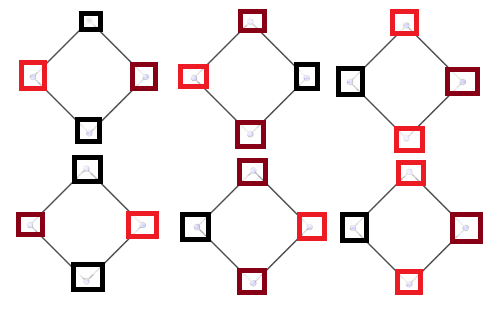
\includegraphics[scale=0.4]{brincos2.png}
\end{center}

Sem listar as possibilidades, pelas observações dadas no item a) e pelo Principio multiplicativo, temos dois casos a considerar, se a diagonal que possui o fecho tem pedras iguais ou diferentes. Se forem iguais, identificamos com uma cor a diagonal do fecho, com 3 possibilidades de cores, e portanto 2 possibilidades a pedra adjacente a direita e uma a pedra adjacente a esquerda, obtendo $3 \cdot 2 \cdot 1=6$ brincos . Caso contrário, as pedras adjacentes ao vértice que contem o fecho deverão ter cores iguais, e de modo análogo construímos $3 \cdot 2 \cdot 1=6$  brincos. Totalizando 12 brincos.
\item Quando a contagem é por bracelete só são as seis soluções apresentadas, não existe a mudança do fecho para gerar as outras soluções. 

\end{enumerate}
}{0}
\end{answer}
\clearmargin
\begin{answer}{Produzindo Acessórios}
{
\begin{enumerate}\setcounter{enumi}{4}
\item São 12 brincos e 6 braceletes. Existem 12 possibilidades para a escolha dos brincos e 6 para a escolha dos braceletes, pelo princípio multiplicativo $12 \cdot 6 = 72$ maneiras diferentes de organizar o conjunto. 
\item São 8 pedras e 3 cores, tendo pelo menos uma pedra de cada cor. 
$$ \circ \circ \circ \circ \circ \circ \circ \circ \circ .$$
O que diferencia os brincos é a quantidade de pedras de cada cor e portanto não importa a ordem que essas pedras aparecem (esquerda para direita ou ao contrário).
Pensando que elas podem ser separadas em 3 conjuntos, as que são pintados da cor 1, as que são pintados da cor 2 e as que são pintados da cor 3, logo dois espaços devem ser inseridos entre as pedras. 
$$ \circ \circ \circ \circ \circ \circ \circ \circ \circ \_ \_ .$$
As pedras que estão antes do espaço 1 são da cor 1, as pedras que são da cor 2 estão entre dois espaços e as pedras da cor 3 estão depois do espaço 2. Como todas as cores devem ser usadas, os dois espaços podem estar em 7 lugares diferentes, logo são 7 possibilidades para escolha do lugar para o primeiro espaço, 6 para a escolha do segundo espaço. Como esses espaços são indistinguíveis é preciso dividir por 2, $\dfrac{7 \cdot 6}{2}= 21$.
\item É possível ainda usar a ideia de pedras e espaços 
$$ \circ \circ \circ \circ \circ \circ \circ \circ \circ \_ \_ .$$
Mas agora é permitido que dois espaços fiquem juntos, ou que a ordem comece ou termine com o espaço, representando não ter pedra de determinadas cores. 
Neste caso são 10 objetos para serem organizados em fila, sendo 8 de um determinado tipo e 2 de outro. O número de maneiras de se fazer isso é dado por $\dfrac{10!}{2!8!}=45.$ (permutação com repetição)
\end{enumerate}
}{1}
\end{answer}

\begin{task}{Produzindo Acessórios}

Para a produção de algumas bijuterias, como brincos e braceletes são usadas pedras de três cores diferentes. Levando em conta três cores, responda:
 
\begin{enumerate}
\item O modelo dos brincos é dado por um quadrado com uma pedra em cada um dos vértices e com o fecho na parte de trás de uma das pedras. 

\begin{figure}[H]
\centering

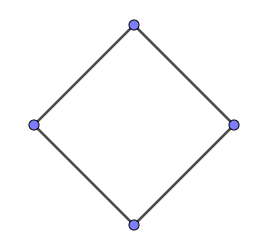
\includegraphics[scale=0.4]{brincos.png}
\end{figure}

Pense em alguns modelos de brinco que usem exatamente as  três cores de pedras disponíveis de modo que duas pedras na sequência não sejam da mesma cor.

\item A turma conseguiu muitos modelos diferentes? Compare seu modelo com o dos amigos.
\item Quantos brincos diferentes é possível produzir levando em conta a restrição das cores dada no item a)?
\item O modelo dos braceletes é dado por 4 peças contendo uma pedra cada igualmente espaçadas.  Quantos braceletes é possível fabricar levando em conta a mesma restrição nas cores?
\item Quantos conjuntos diferentes com um par de brincos e um bracelete é possível formar? Eles não precisam necessariamente ter a mesma organização nas cores.
\item Pensando em outro modelo de brinco, formado por 8 pequenos pêndulos com uma pedra em cada, não faz mais sentido pensar na restrição para as cores lado a lado. O que diferencia uma bijuteria da outra agora é a quantidade de pedras de uma determinada cor. Supondo ainda que temos que ter pedras das três cores disponíveis,  quantas peças diferentes deste tipo é possível produzir?  
\item E se na produção dos brincos em pêndulos fosse permitido agora ter até 3 cores e não mais exatamente 3 cores? 
      
 \end{enumerate}
\end{task}

\clearmargin
\def\currentcolor{session2}
\begin{objectives}{Hora de criar}
{
\begin{itemize}
\item Criar problemas de contagem considerando certas restrições.
\item  Criar uma classificação pessoal para os vários tipos de problemas.
\end{itemize}
}{1}{1}
\end{objectives}
\begin{sugestions}{Hora de criar}
{
O esperado para esta atividade é que os estudantes usem dos exercícios anteriores e criem situações se colocando como autores e espectadores de ações de contagem. Uma possibilidade é sugerir problemas envolvendo jogos como truco, dados ou xadrez.
}{1}{1}
\end{sugestions}
\begin{answer}{Hora de criar}
{
\begin{enumerate}
\item Questões criadas nesse item podem ser simples como : de quantas maneiras podemos escolher um sabor e uma cobertura de sorvete entre dez diferentes sabores de sorvete e três tipos de cobertura? Se tomar sorvete não é algo muito ao estudante  a mesma questão pode ser adaptada a uma situação de escolha do cotidiano dele, claro, envolvendo conjuntos disjuntos.
\item Algumas sugestões são problemas que envolvam criar grupos, subgrupos, comissões, reuniões de amigos e times.
\item Algumas sugestões são problemas que envolvam colocar pessoas em ciranda, rodas de oração, sentadas em roda para as mais diversas situações como jantares, roda de conversa, para jogar baralho e outros jogos, assim como confeccionar objetos circulares como a braceletes.
\item Para criar essa questão, uma situação pode ser criada e vários itens de contagem como cada restrição podem ser pedidos, como por exemplo o questionamento feito na seção 1.1 sobre criação de grupos com variadas situações e restrições.
\item Pergunte aos estudantes as estratégias utilizadas e discuta as estratégias possíveis com a turma para os problemas criados. 
\end{enumerate}
}{1}
\end{answer}
\arrange{Contando agrupamentos}

Voltemos ao questionamento proposto no início da seção. O número de maneiras de se retirar 3 bolas amarelas e 2 vermelhas de uma urna com 5 bolas, sem reposição, tem alguma relação com o número de maneiras de se escolher 3 pessoas de um grupo de 5? Apesar de serem agrupamentos diferentes:  o primeiro temos um agrupamento de 5 bolas com repetição das bolas amarelas (aparecem 3 vezes) e repetição das bolas vermelhas (aparecem 2 vezes); já o segundo é um conjunto de 3 pessoas escolhidas dentre 5 pessoas distintas, a solução de ambos os problemas é a mesma, $\dfrac{5!}{2!3!}.$
Assim, é difícil caracterizar todos os problemas e tipos de agrupamentos existentes por meio de suas soluções. Não existe um passo a passo pré-definido para a resolução de todos os problemas de contagem, cada um deve ser lido, interpretado e os passos construídos de maneira específica, é preciso se imaginar resolvendo o problema. Os cálculos seguem a mesma linha dos passos organizados, cada etapa definida corresponde a uma parte da solução.  Ao pensar na solução para um problema de contagem alguns questionamentos devem ser feitos:

\begin{enumerate}

    \item O problema tem algum tipo de restrição?
    
    As restrições devem ser consideradas primeiro, caso isso não seja feito pode ser que sua solução fique muito complicada.

    \item É preciso quebrar o problema em casos mais simples?
    
    Alguns problemas parecem muito difíceis a primeira vista, mas quando interpretados com cuidado podem ser divididos em casos menores cuja resolução seja mais simples. (\textbf{Princípio Aditivo})
    
    \item O referencial escolhido está correto?
    
    Os problemas podem ser resolvidos por diferentes caminhos, tomando diferentes referenciais para contagem. Algumas escolhas deixam o problema mais difícil por conta do número de casos a se considerar. 
    
    \item Os elementos que compõe a contagem fazem parte de conjuntos disjuntos (conjuntos que não possuem elementos comuns)?
    
    Se o \textbf{Princípio Multiplicativo} é usado para contagem de sucessivos elementos tomados em conjuntos disjuntos ele não impõe ordem. Caso contrário, se o agrupamento for tomado no mesmo conjunto, sua utilização impõe ordem. 
    
    \item Os objetos contados são distintos? 
    
    Existe a possibilidade de ter disponível várias cópias do mesmo objeto para a composição dos agrupamentos.
    
    \item A repetição dos elementos na contagem é permitida?
    
    O problema pode descrever elementos distintos, mas que podem ser repetidos.

    \item Todos os elementos disponíveis precisam ser usados?
    
    Alguns agrupamentos usam todos os elementos do conjunto outros usam parte deles. 
    
    \item A estratégia escolhida realmente conta cada um dos casos uma única vez? 
    
    Depois de pensar no caminho para a solução é preciso refletir se realmente todos os elementos de interesse foram contados uma única vez. Essa mesma reflexão pode ser feita a fim de verificar se existem elementos contados a mais ou a menos.
    
\end{enumerate}

\practice{Contando Agrupamentos}

\begin{task}{Hora de criar}
Nas Atividades desenvolvidas foi possível perceber a variedade de situações e técnicas de resolução de problemas de contagem. Agora é a hora de criar os seus problemas. Vocês podem manter todos os problemas em torno de uma única temática ou variar os assuntos abordados. Mãos à obra!

\begin{enumerate}

    \item Crie um problema de contagem que envolva dois conjuntos disjuntos; 
    \item Crie um problema de contagem no qual a ordem dos elementos no agrupamento não seja importante;
    \item Crie um problema de contagem que envolva organizar elementos em roda;
    \item Crie um problema de contagem em que todos os itens anteriores sejam satisfeitos. 
    \item Agora resolva os problemas criados por outros grupos. As ideias foram parecidas?
    
\end{enumerate}
\end{task}

\clearpage
\def\currentcolor{session3}
\begin{texto}
{
\subsection{Generalizando}\small
\cite{Renan} relatam em sua pesquisa a dificuldade que os estudantes apresentam em compreender as fórmulas relativas aos problemas de contagem, desde não saberem qual fórmula usar até mesmo na substituição dos termos. Ou seja, é realmente confuso para eles o uso. As fórmulas são generalizações do que foi desenvolvido do raciocínio combinatório, portanto é importante que os estudantes percebam que elas foram construídas com os mesmos argumentos usados na própria resolução da atividade. 

Nas seções anteriores os estudantes foram levados a pensar em agrupamentos com certo número de elementos, esse número foi modificado de forma que a turma percebesse as regularidades, sendo capazes de pensar no caso geral.
No entanto, acredita-se que as fórmulas não devem ser o foco do estudo de Análise Combinatória. Esse estudo deve estar centrado nas interpretações e uso do Princípio Aditivo e do Princípio Multiplicativo. Se ainda assim as fórmulas estiverem disponíveis ao uso, é preciso que se tenha clareza de como elas podem ser utilizadas. 

A simbologia utilizada nos casos gerais  tem relevância em algumas situações. Por exemplo, a prova do ENEM e alguns vestibulares exige o conhecimento dos símbolos referentes a contagem de agrupamentos; eles aparecem como resposta das alternativas dos problemas e, neste caso, não adiantaria resolver o problema sem ser capaz de identificar no gabarito a resposta correta. 

Neste contexto, a proposta é que os estudantes trabalhem na elaboração de uma Calculadora  Combinatória: que agrupamentos a calculadora poderia considerar? Que dados precisa de entrada? Quais problemas consegue resolver? Neste momento surgirá a necessidade de se pensar no caso geral. Cada grupo poderá construir uma calculadora diferente, dependendo dos dados de entrada. Nesta elaboração vão precisar deduzir as fórmulas para os agrupamentos e podem compreender melhor que mesmo tendo uma calculadora em mãos é necessário interpretar e organizar o raciocínio de resolução dos problemas. A calculadora serviria apenas para facilitar os cálculos, não é possível (ainda) transferir para uma máquina todas as nuances de um problema de contagem. 

Muitos autores reforçam o estudo dos problemas de contagem com foco no Princípio Aditivo e Multiplicativo, mas não negam a importância do conhecimento das fórmulas: ``É importante destacar que uma abordagem que não priorize as fórmulas não significa que as negue. As fórmulas se tornam um resultado de processos de reflexão, generalização e sistematização, após o aluno compreender todas as etapas". \cite[p. 53]{Diogo} 

Caso a turma tenha muita dificuldade para deduzir as fórmulas o professor pode exemplificar os agrupamentos com alguns números específicos e realizar modificações até que entendam o caso geral. 
}
\end{texto}
\begin{objectives}{Calculadora Combinatória}
{
Identificar os agrupamentos comuns, conhecer as fórmulas e suas notações;
}{1}{2}
\end{objectives}
\begin{sugestions}{Calculadora Combinatória}
{
O esperado para esta atividade é que os estudantes reflitam sobre os agrupamentos estudados e cheguem a expressão matemática das fórmulas. As explicações dadas abaixo não devem ser apresentadas a eles inicialmente, o que pode ser feito é orientá-los que façam as contas com números menores, variem os números e percebam a regularidade até a generalização.

Por exemplo, considere contar o número de  arranjos possíveis de três elementos dentre os elementos do conjunto de $5$ elementos distintos $\{1,2,3,4,5\}.$ Isso por ser feito usando o Principio Multiplicativo obtendo $5 \cdot 4 \cdot 3$ maneiras possíveis. Considere agora contar o número de arranjos possíveis de três elementos dentre os elementos do conjunto de $6$ elementos distintos $\{1,2,3,4,5,6\}.$ Isso por ser feito usando o Principio Multiplicativo obtendo $6 \cdot 5 \cdot 4 $ maneiras possíveis. Faça esse mesmo raciocínio até chegar a um conjunto com $7$ elementos (talvez mais se não se sentir exaustivo), e depois coloque os resultados em fileira: 

$$5 \cdot 4 \cdot 3,$$
$$6 \cdot 5 \cdot 4,$$
 $$7 \cdot 6 \cdot 5.$$

Agora, seguindo essa linha e colocando um conjunto com $n$ elementos, indague como ficaria essa mesma expressão, obtendo $$n \cdot (n-1) \cdot (n-2).$$   Interpretando, a expressão obtida significa, como todos os outros anteriores obter o número de arranjos de 3 elementos dentre um conjunto de $n$ elementos distintos $\{1,2, \cdots, n\}.$ Agora pergunte aos alunos qual a relação do número $3$ com a expressão obtida ? A resposta é o número de parcelas que estão sendo multiplicadas, começando pelo $n$ e diminuindo em uma unidade cada até chegar nesse número de parcelas. Quem seria a última parcela? Neste caso temos $n-2=n-(3-1).$ Agora trocando o número $3$ por uma incógnita $p$ teríamos então $p$ parcelas que estão sendo multiplicadas, começando pelo $n$ e diminuindo em uma unidade cada até chegar nesse número de parcelas. Quem seria a última? Neste caso temos $n-(p-1)=n-p+1.$ Assim, conseguimos generalizar e determinar $$A_n^p=n (n-1)(n-2)(n-3) \cdots (n-p+1).$$
}{0}{0}
\end{sugestions}
\begin{answer}{Calculadora Combinatória}
{
\begin{enumerate}
\item A calculadora deve ter botões com números de $0$ a $9,$ botões com as operações básicas de soma, subtração, divisão e multiplicação e botão com sinal de igualdade para obter as respostas. Também poderá conter um botão para cálculo de fatorial e outro para  o cálculo de potência de números. 
\setcounter{enumi}{2}
\item O desenho será diversificado e pode ser melhorado após o compartilhamento com a turma.
\end{enumerate}
}{1}
\end{answer}
\begin{answer}{Calculadora Combinatória}
{
\begin{enumerate}\setcounter{enumi}{1}
\item Podem ser incluídos botões que calculem a quantidade de arranjos, combinações e permutações, além dos agrupamentos com repetição.  Cada um desses botões devem ter descritas suas fórmulas gerais e ter como entrada os dados necessários para o cálculo.

Seguem alguns comentários para ajudar na compreensão das fórmulas.

O Arranjo é um agrupamento com elementos diferentes. Considerando um conjunto com $n$ elementos distintos, encontrar o número total de arranjos com $p$ destes elementos pode ser pensado pelo princípio multiplicativo. São $n$ possibilidades para a escolha do primeiro elemento, $n-1$ para o segundo, $n-2$ para o terceiro, $n-3$ para o quarto e $n-(p-1)=n-p+1$ para o $p$ -ésimo. Assim, obtém-se pelo Princípio Multiplicativo que o número total de arranjos é dado por 
\small
\begin{align*}
A_n^p&=n (n-1)(n-2)(n-3) \cdots (n-p+1)\\
&= \dfrac{n (n-1)(n-2)(n-3) \cdots (n-p+1)(n-p) (n-(p+1)) (n-(p+2))\cdots 1}{(n-p) (n-(p+1)) \cdots 1} \\
&= \dfrac{n!}{(n-p)!}.
\end{align*}
\normalsize
A permutação é um embaralhamento dos elementos, também pode ser pensada como um arranjo com $n=p$, com isso, o número de permutações de $n$ elementos distintos é igual a 
$$P_n=n!.$$

Ainda pode ser olhara para a permutação como o número de maneiras de organizar os objetos em fila e, neste caso, usando o princípio multiplicativo, para a primeira posição são $n$ possibilidades, para a segunda $n-1$, seguindo assim até a última posição com 1 possibilidade. 


Usando a permutação, é possível verificar que a manipulação algébrica feita no arranjo para se chegar a fórmula nada mais é do que organizar as $n$ pessoas em fila, considerar as $p$ primeiras e dividir pelo número de filas que possuem esses $p$ primeiros elementos, ou seja, dividir por todas as filas formadas por $(n-p)$ elementos que se referem a parte que não será considerada. 

A combinação se refere a um agrupamento onde a ordem dos elementos distintos não importa, e está ligada ao ato de escolher. 
A dedução da sua fórmula se inicia como do arranjo, mas como a ordem não é importante é preciso retirar as repetições de agrupamentos formados. Um conjunto com $p$ elementos pode ser organizado de $p!$ maneiras diferentes em fila, logo foram contabilizadas $p$ cópias de cada solução e por esse motivo deve ser dividido por $p!$. Assim o número de combinações de $p$ elementos dentre $n$ elementos distintos é dado por
\small
\begin{equation*}
C_n^p=\dfrac{A_n^p}{p!}= \dfrac{n!}{p!(n-p)!}.
\end{equation*}
\normalsize
Espera-se que eles coloquem na calculadora os botões dos números, operações básicas, potenciação e até possivelmente, símbolos que contenham fórmulas ligadas aos agrupamentos que criaram. 
\end{enumerate}
}{0}
\end{answer}
\begin{objectives}{Testando a Calculadora Combinatória}
{
\begin{itemize}
\item Utilizar as fórmulas e notações para contagem dos vários tipos de agrupamentos. 
\item Observar que antes da utilização da fórmula vem a interpretação do problema
\end{itemize}
}{1}{1}
\end{objectives}
\begin{sugestions}{Testando a Calculadora Combinatória}
{
O esperado para esta atividade é que os estudantes consigam criar uma solução para o problema e depois descrevam a sequência de botões em sua calculadora. A solução apresentada aqui é apenas uma das possibilidades que podem surgir na sala. 

\textbf{Tempo de Execução:} A questão pode ser feita em 30  minutos sendo utilizados de 5 a 10 minutos para cada item. 
}{1}{1}
\end{sugestions}
\begin{answer}{Testando a Calculadora Combinatória}
{
\begin{enumerate}
\item 
\adjustbox{valign=t}
{
\begin{tabular}{|>{\centering}m{.5\linewidth}|c|}
\hline
\tcolor{Ações para solução}  & \tcolor{Tradução matemática} \\
\hline
$A_1$: Escolher dois jogadores quaisquer  & $C_{10}^2$\\
\hline
$A_2:$ Escolher dois jogadores canhotos & $C_{4}^2$ \\
\hline
$A_3:$ Retirar do total de duplas as duplas só de canhotos & $C_{10}^2 - C_{4}^2.$\\
\hline
\end{tabular}
}

ou 

\begin{tabular}{|>{\centering}m{.5\linewidth}|c|}
\hline
\tcolor{Ações para solução}  & \tcolor{Tradução matemática} \\
\hline
$A_1$: Escolher equipes só com destros  & $C_{6}^2$\\
\hline
$A_2:$ Escolher um destro & $C_{6}^1$ \\
\hline
$A_3:$ Escolher um canhoto & $C_{4}^1$\\
\hline
$A_4:$ Princípio Multiplicativo em $A_{2}$ e $A_{3}$  & $C_{6}^1 \cdot C_{4}^1$\\
\hline
$A_5:$ Princípio Aditivo em $A_1$ e $A_4$  & $C_{6}^2  + C_{6}^1 \cdot C_{4}^1 .$\\
\hline
\end{tabular}     

\item Observe que o exercício não especifica se a repetição é permitida ou não. Neste caso, usamos sempre que a repetição é permitida, caso não fosse, o exercício deveria deixar explícito essa restrição.

\begin{tabular}{|>{\centering}m{.5\linewidth}|c|}
\hline
\tcolor{Ações para solução}  & \tcolor{Tradução matemática} \\
\hline
$A_1$: Escolher onde colocar as letras  & $C_{4}^2$\\
\hline
$A_2:$ Alocar as letras nos locais escolhidos  & ${52}^2$ \\
\hline
$A_3:$ Alocar os algarismos nos espaços faltantes & ${10}^2$\\
\hline
$A_4:$ Princípio Multiplicativo & $C_{4}^2  \cdot {52}^2 \cdot {10}^2$\\
\hline
\end{tabular}

\item
\adjustbox{valign=t}
{
\begin{tabular}{|>{\centering}m{.5\linewidth}|c|}
\hline
\tcolor{Ações para solução}  & \tcolor{Tradução matemática} \\
\hline
$A_1$: Equipe de música com 1 cantor  & $C_{3}^1\cdot C_{7}^3 $\\
\hline
$A_2:$ Equipe de música com 2 cantores  & $C_{3}^2\cdot C_{7}^2$ \\
\hline
$A_3:$ Equipe de música com 3 cantores & $C_{3}^3\cdot C_{7}^1$\\
\hline
$A_4:$ Princípio Aditivo  em $A_{1},A_{2}$ e $A_{3}$ & $C_{3}^1\cdot C_{7}^3+ C_{3}^2\cdot C_{7}^2+ C_{3}^3\cdot C_{7}^1 $
\\
\hline
\end{tabular}
}

ou

\begin{tabular}{|>{\centering}m{.5\linewidth}|c|}
\hline
\tcolor{Ações para solução}  & \tcolor{Tradução matemática} \\
\hline
$A_1$: Equipe com 4 membros quaisquer  & $C_{10}^4 $\\
\hline
$A_2:$ Equipe de música sem cantores & $C_{7}^4$ \\
\hline
$A_3:$ Retirar do total equipes só com músicos & $C_{10}^4- C_{7}^4$\\
\hline
\end{tabular}
\end{enumerate}
}{0}
\end{answer}
\know{Generalizando}

\paragraph{Para que servem as calculadoras?}

\begin{center}
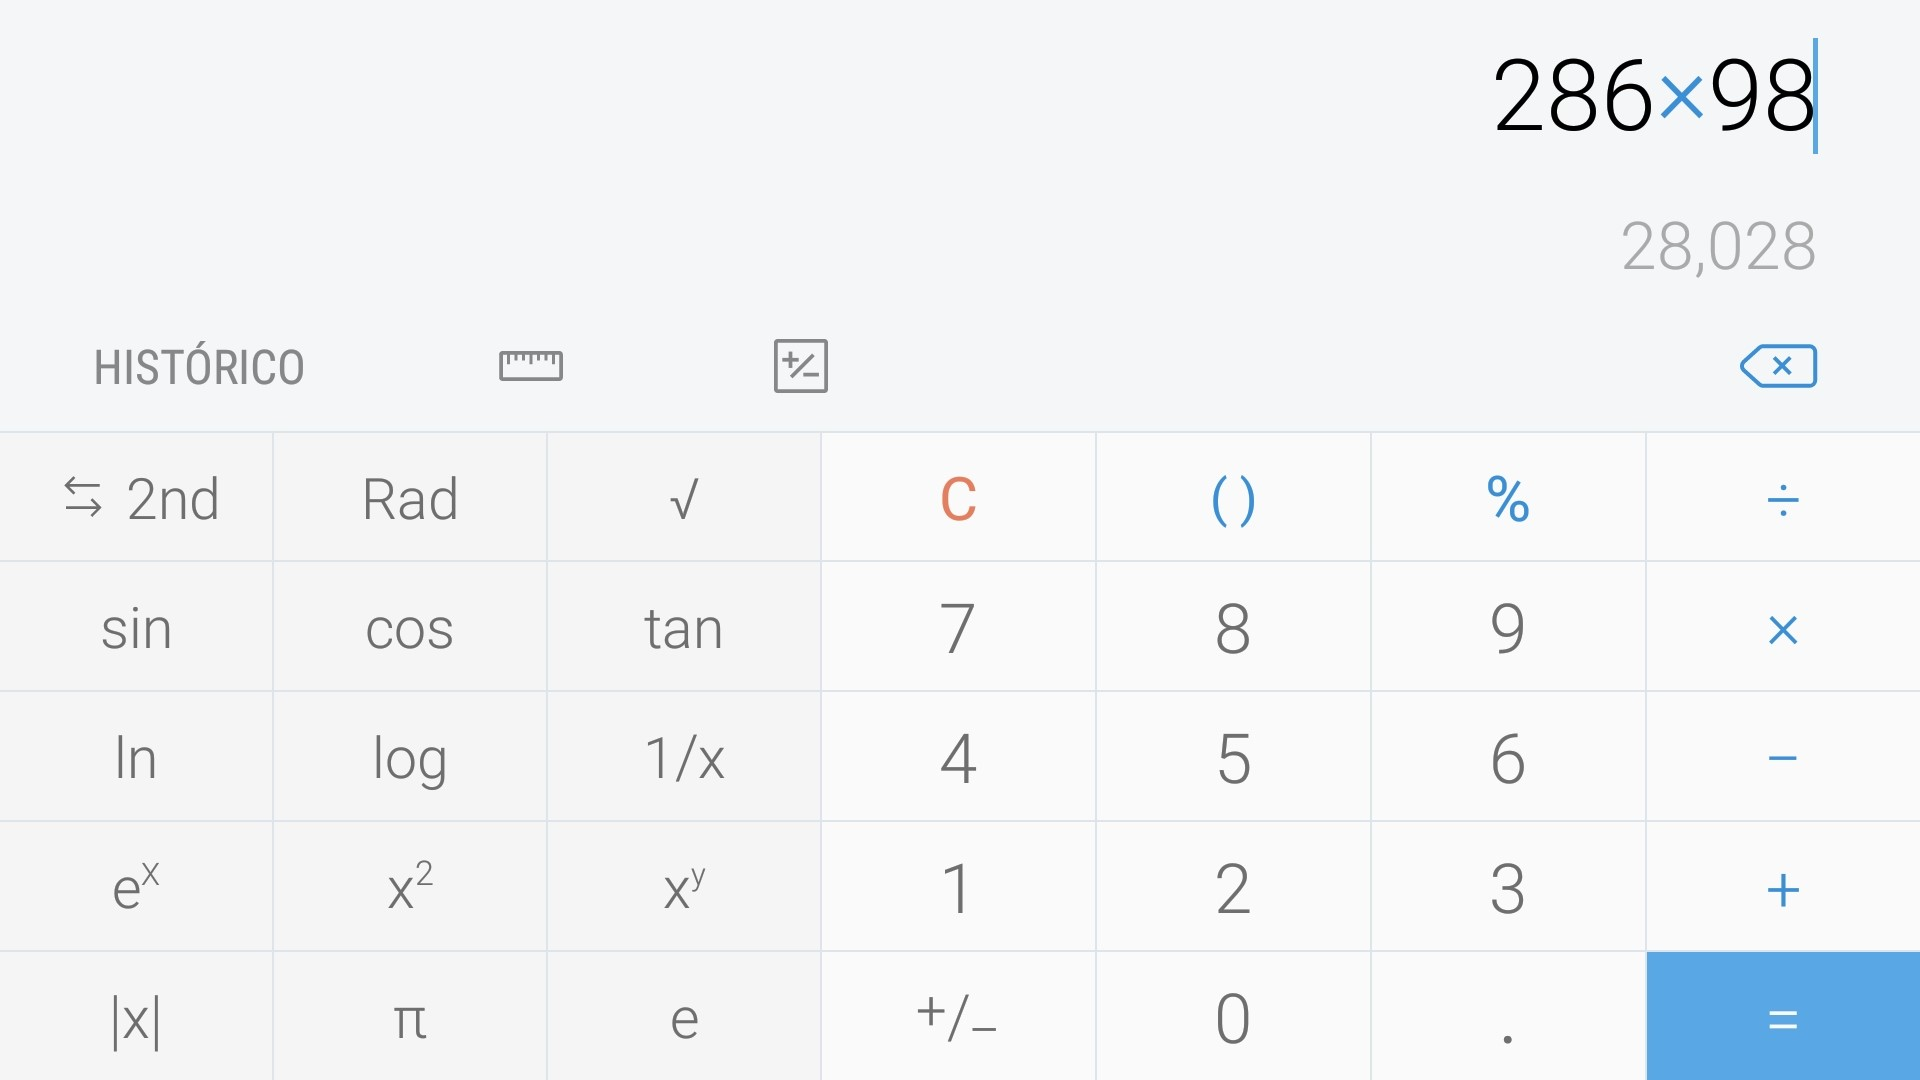
\includegraphics[scale=0.18]{calculadora.jpeg}
\end{center}

Vocês já pararam para pensar no surgimento da primeira calculadora? 
Hoje existem no mercado vários tipos delas, online ou não, desde as mais simples até as mais sofisticadas. Estão presentes até nos aparelhos celulares. Pra que elas servem? Elas ajudariam a solucionar os problemas pensados neste livro?

\begin{task}{Calculadora Combinatória}
Uma calculadora não é capaz de resolver os problemas do cotidiano, mas ela pode diminuir e muito o tempo de realização dos cálculos. Sabendo como usar, ela é uma forte aliada nas tarefas do dia a dia. Projete com seus colegas de grupo uma Calculadora Combinatória.



Os agrupamentos mais comuns estão descritos abaixo, mas o grupo pode pensar outras organizações possíveis e úteis de acordo com sua percepção dos problemas estudados no material.

\begin{itemize}
\item \textbf{Arranjo:}  é uma maneira de organizar em fila parte dos elementos de um determinado conjunto de elementos distintos. Considerando o conjunto $\{1,2,3,4,5\}$, o número 253 é um arranjo formado por três elementos deste conjunto com cinco elementos, que é diferente do arranjo 532. Neste caso os arranjos são diferentes e a ordem em que os elementos estão organizados é importante, trocar a ordem de elementos significa gerar outro arranjo com os mesmos elementos. A notação para o número de arranjos possíveis com $p$ elementos de um conjunto com $n$ elementos distintos é  dada por $A_n^p$ ou  $A_{n,p},$ 


\item \textbf{Permutação:} é um embaralhamento de elementos distintos. Leva em conta elementos distintos e se refere a organização deles em fila. Pode ser considerado um arranjo de todos os elementos do conjunto. Comumente usa-se a notação $P_n$ para o número de permutações de $n$ objetos. 


\item \textbf{Combinação:} é um subconjunto de um conjunto de elementos distintos. Ou ainda, um agrupamento formado pela escolha de elementos de um conjunto dado. Por exemplo, considerando o conjunto $\{1,2,3,4,5\}$, uma combinação formada por três elementos dele é dada por $\{2,5,3\}$. A ordem da escolha não interfere no subconjunto criado, apenas leva em conta que os elementos são distintos.  Notação normalmente usada $C_n^p,C_p^n$ ou ainda, $C_{n,p}$ para o número de combinações possíveis com $p$ elementos de um conjunto com $n$ elementos. 


\item \textbf{Agrupamento com repetição:} é um agrupamento tomado em um conjunto que possua várias cópias de determinados objetos, ou que um mesmo elemento possa ser usado mais de uma vez. Exemplos: 121 é um tipo de arranjo dos algarismos que permite a repetição.  Escolher duas bolas vermelhas e uma azul de uma urna contendo 3 bolas vermelhas, 4 bolas azuis e 2 amarelas é um agrupamento com objetos repetidos. É possível considerar permutação, arranjo e combinação com repetição. 
\end{itemize}


\begin{enumerate}
\item Quais botões a calculadora precisa ter para resolver os problemas os problemas de contagem estudados aqui? 

\item Quais botões podem ser incluídos a calculadora para incluir a contagem dos agrupamentos comuns estudados aqui? Como incluir a possibilidade de repetição de objetos?


\item Faça um desenho que represente a calculadora e explique a funcionalidade de cada um dos botões.

\end{enumerate}
\end{task}

\begin{task}{Testando a calculadora combinatória}
Nos problemas a seguir escreva uma solução e descreva a sequência de botões, na sua calculadora, que seria necessária para encontrar a solução correta.

\begin{enumerate}
\item (Enem 2016, adaptada) O tênis é um esporte em que a estratégia de jogo a ser adotada depende, entre outros fatores, de um adversário ser canhoto (joga usando a mão esquerda) ou destro (joga usando a mão direita). 

Um clube tem um grupo de 10 tenistas, sendo que 4 são canhotos e 6 são destros. O técnico do clube deseja realizar uma partida de exibição entre dois desses jogadores, porém não poderão ser ambos canhotos. Qual o número de possibilidades de escolha dos tenistas para a partida de exibição.  

\item (Enem 2016, adaptada) Para cadastrar-se em um \textit{site}, uma pessoa precisa escolher uma senha composta por quatro caracteres, sendo dois algarismos e duas letras (maiúsculas ou minúsculas). As letras e algarismos podem estar em qualquer posição. Essa pessoa sabe que o alfabeto é composto por vinte e seis letras e que uma letra maiúscula difere da minúscula em uma senha. 
 {Disponível em: www.infowester. com. Acesso em 14 dez. 2012.}
 
Qual o número total de senhas possíveis para o cadastramento nesse site?

\item Em uma escola de música, 7 professores tocam algum instrumento e outros 3 cantam. Ocorrerá uma festa onde 4 dos 10 serão contratados, com pelo menos 1 que cante. Quantas equipes podem ser formadas?

\end{enumerate}
\end{task}

Algumas características de problemas combinatórios são comuns, o que torna possível organizá-los em alguns tipos de agrupamentos: arranjos, permutações e combinações, com ou sem repetições. As fórmulas nada mais são do que o resumo da contagem para cada tipo de agrupamento. Mas saber apenas as fórmulas não significa conseguir resolver um problema de contagem. As ideias trabalhadas neste material seguiram no sentido de discutir algumas possibilidades de solução e apresentar maneiras de organização do raciocínio, mas para resolver um problema de contagem é necessário realmente traçar um passo a passo de ações que podem ser traduzidas em operações matemáticas.
Os verbos que mais aparecem são  escolher, permutar e arranjar, mais fortemente escolher e permutar. 

Escolher se refere ao ato de tomar um subconjunto de um conjunto dado, neste ato não importa em que ordem essa escolha foi feita, importa apenas quais elementos foram escolhidos. Permutar é equivalente ao ato de  embaralhar ou enfileirar os elementos. Arranjar por outro lado se refere a um embaralhamento de elementos escolhidos, ou de embaralhamento de parte dos elementos de um conjunto. Escolher e depois embaralhar é equivalente a arranjar. Assim, o número de arranjos de $p$ elementos dentre $n$ elementos distintos é calculado se escolhermos $p$ dentre $n$ elementos possíveis, e depois multiplicar esse valor pela permutação desses $p$ elementos. 

Na linguagem matemática podemos escrever

\begin{align*}
A_n^p&= p! \cdot C_n^p,\\
C_n^p&= \dfrac{A_n^p}{p!}.
\end{align*}

Mais do que fórmula, é importante reconhecer os usos do Princípio Aditivo e Multiplicativo. Resolver um problema combinatório é realizar uma sequência de passos que leva em conta esses três atos: escolher, permutar (ou embaralhar) e arranjar, combinados com as operações básicas.

\clearpage
\def\currentcolor{cor1}
\mspace{.25em}
\begin{answer}{Exercícios}
{\exerciselist
\begin{enumerate}
\item É importante que os estudantes consigam perceber que não importa de qual tipo são os  elementos que estão sendo organizados, o relevante é que todos os elementos são distintos e devem aparecer na organização uma única vez. 

A solução para os três questionamentos é dado por $P_6 =6!$, pois existem 6 possibilidades de escolha do elemento que ocupará a primeira posição, 5 para o segundo, 4 para o terceiro, 3 para o quarto, 2 para o quinto e 1 para o sexto, sejam eles letras, pessoas ou números.
O último deles existe para se discutir com o estudante que não faz diferença se os números a serem permutados são $1, 2, 3, 4, 5$, como normalmente aparece, ou os números dados no exercício.

\item Neste exercício os estudantes podem listar todas as possibilidades e verificar que com $BBFF$ o número de permutações é menor do que as permutações feitas com quatro elementos distintos. Podem listar as permutações com $BB_1FF_1$, que seriam:
\begin{table}[H]
\centering
\small

$\begin{array}{cccc} BB_1FF_1 & B_1BFF_1 & BB_1F_1F & B_1BF_1F \\ 
FF_1BB_1  & F_1FBB_1  & FF_1 B_1B  & F_1FBB_1 \\
    
BFB_1F_1 & B_1FBF_1&  BF_1B_1F& B_1F_1BF \\

FBF_1B_1  &  F_1BFB_1  &  FBF_1B_1  & F_1B_1FB \\

    BFF_1B_1  &B_1FF_1B  & BF_1FB_1  & B_1F_1FB \\
    
    FBB_1F_1  & F_1BB_1F &  FB_1BF_1 & F_1B_1BF
\end{array}$
\end{table}
Depois devem ser levados a perceber que em cada uma das linhas a permutação é a mesma se o $B$ for considerado igual a $B_1$ e $F$ igual a $F_1$, ou seja: 

\small
$$BBFF, FFBB, BFBF, FBFB, BFFB, FBBF. $$ 
\normalsize

A solução seria então $\dfrac{24}{4} =6. $

Pois, cada coluna da tabela corresponde a uma cópia da solução do problema, como são 4 colunas  a solução deve ser o total de elementos da tabela dividido pelo número de colunas.
Os estudantes podem realizar a contagem fazendo como apresentado, imaginando que são 4 letras distintas e depois descontando as repetições ou pode organizar uma listagem para contar todos os casos. 
Ainda, usando os tipos de agrupamentos existentes, esse exercício pode ser considerado um caso de contagem de todas as  permutações com repetição, logo podemos contar todas as permutações de $4$ letras, dando $4!=24$ e depois retirar as repetições (equivalente a fazer a divisão). Nesse caso, cada dar de letras se repete duas vezes, logo devemos ter $2!2!$ cópias de cada solução. Assim, obtemos o mesmo resultado $\dfrac{24}{2!2!} =6. $
\end{enumerate}
}{1}
\end{answer}
\begin{answer}{Exercícios}
{\exerciselist
\begin{enumerate}\setcounter{enumi}{2}
\item A turma tem 40 alunos e o total de equipes é 5, logo cada equipe deve ter 8 estudantes cada. Seguindo a divisão como apresentada acima para a escolha dos membros da equipe amarela existem: 

40 possibilidades para escolha do primeiro membro, 39 para o segundo, 38 para o terceiro, 37 para o quarto, 36 para o quinto, 35 para o sexto, 34 para o sétimo e 33 para o oitavo. 

Então : $40 \cdot 39 \cdot 38 \cdot 37 \cdot 36 \cdot 35 \cdot 34 \cdot 33$ possibilidades para a escolha do primeiro, seguida do segundo, seguida do terceiro, seguida do quarto, seguida do quinto, seguida do sexto, seguida do sétimo, seguida do oitavo. Mas levando em conta que os mesmos 8 escolhidos em qualquer outra ordem formam a mesma equipe essas repetições precisam ser retiradas da contagem anterior. O número de maneiras de organizar 8 pessoas em fila é dado por $8!$, ou seja, uma única equipe foi contadas $8!$ na contagem inicial, logo a solução para o problema é dado por: 

$\dfrac{40 \cdot 39 \cdot 38 \cdot 37 \cdot 36 \cdot 35 \cdot 34 \cdot 33}{8!} = 76904685$ maneiras diferentes. 

Ainda, usando os tipos de agrupamentos existentes, esse exercício pode ser considerado um caso de contagem de todas as  combinações de 8 elementos dentre 40 elementos distintos. Isso pode ser feito determinando todos os arranjos de 8 dentre 40 elementos distintos e depois retirando as repetições pois se trata de um subconjunto não ordenado (equipe). Assim, temos  $$C_{40}^8=  \dfrac{A_{40}^8}{8!} = \dfrac{40 \cdot 39 \cdot 38 \cdot 37 \cdot 36 \cdot 35 \cdot 34 \cdot 33}{8!} = 76904685.$$

\item Este problema possui uma restrição que deve ser o ponto inicial de atenção. Começando escolhendo a camiseta amarela o cenário de possibilidades é diferente de se pensar em qualquer outra camiseta. Para evitar cálculos errados, esse problema precisa ser dividido em dois problemas menores. Contar o número de uniformes que levem em conta a camiseta amarela e os que não a admitem. Essas duas condições são disjuntas, não tem como uma camiseta ser amarela e não amarela ao mesmo tempo. Com isso a solução do problemas é a soma das soluções encontradas.
Começando com uma camiseta amarela, existem 3 possibilidades de bermudas: azul, preta e cinza. Agora contar os uniformes que não tenham camiseta amarela, seriam 2 possibilidades para a escolha da camiseta vezes 4 possibilidades de escolha das bermudas, o que resulta em 8 possibilidades. 
Com isso o número total de uniformes seria 8+3=11. 

Este problema também poderia ser solucionado contando todos os possíveis uniformes que seriam: $3\cdot 4 =12$ e retirando a única opção que é a camiseta amarela com bermuda amarela. 

Como o número de elementos envolvidos neste problema ainda é pequeno, é provável que alguns estudantes decidam por listar todos os casos. 

\columnbreak
\item Fixando uma ordem para os grupos: amarela, vermelha, laranja, branca e preta.

~~

$\dfrac{40 \cdot 39 \cdot 38 \cdot 37 \cdot 36 \cdot 35 \cdot 34 \cdot 33}{8!}$ - Maneiras de escolher o primeiro grupo. A divisão por $8!$ foi feita pois cada equipe de oito pessoas possíveis foi contada $8!$ vezes.  

~~


$\dfrac{32 \cdot 31 \cdot 30 \cdot 29 \cdot 28 \cdot 27 \cdot 26 \cdot 25}{8!}$ - Maneiras de escolher o segundo grupo. Para cada escolha de oito para primeiro restam 32 para estarem na segunda equipe. 

~~


$\dfrac{24 \cdot 23 \cdot 22 \cdot 21 \cdot 20 \cdot 19 \cdot 18 \cdot 17}{8!}$ - Maneiras de escolher o terceiro grupo. Para cada escolha de oito para o segundo restam 24 para estarem no terceiro grupo. 

~~


$\dfrac{16 \cdot 15 \cdot 14 \cdot 13 \cdot 12 \cdot 11 \cdot 10 \cdot 9}{8!}$ - Maneiras de escolher o quarto grupo. Para cada escolha de oito para o terceiro restam 16 para estarem no quarto grupo. 

~~

$\dfrac{8 \cdot 7 \cdot 6 \cdot 5 \cdot 4 \cdot 3 \cdot 2 \cdot 1}{8!}$ - Maneiras de escolher o quinto grupo. Para cada escolha de oito para quarta restam 8 para estarem no quinto grupo, ou seja, escolhendo o quarto grupo o quinto é escolhido automaticamente.

Pelo Princípio Multiplicativo,  $\dfrac{40!}{8!^5}$ maneiras diferentes de dividir os 40 alunos em 5 grupos. 

Para responder ao problema inicial é preciso contar, o número de grupos possíveis em que as amigas estejam juntas, elas podem retirar a mesma fita de $5$ maneiras diferentes, para cada uma dessas maneiras as outras equipes serão recompostas entre os $38$ alunos restantes, mas uma destas cores receberá apenas $6$ membros novos. Seguindo o raciocínio para contar o caso geral seria: $ 5 \cdot \dfrac{38!}{6!\cdot 8!^4}.$

Com isso teriam o quociente de todos os casos favoráveis por todos os casos possíveis: 

$$\dfrac{5 \cdot \dfrac{38!}{6!\cdot 8!^4}}{\dfrac{40!}{8!^5}} = \dfrac{5 \cdot 38! \cdot 8!}{6!40!}= \dfrac{7}{39}.$$ O que equivale a


7 chances em 39 de estarem na mesma equipe. 
Pensando em linguagem de agrupamentos, determinar equipes é determinar combinações, ou ainda, subconjuntos de um conjunto com elementos distintos. Assim, fixando uma ordem para os grupos: amarela, vermelha, laranja, branca e preta, teríamos o número total de agrupamentos dado por 
$$C_{40}^8C_{32}^8C_{24}^8C_{16}^8C_{8}^8 =\dfrac{40!}{8!^5} .$$
Agora, observamos que as amigas podem estar juntas de $5$ maneiras diferentes, devemos contar as combinações possíveis se estiverem na equipe amarela, depois as combinações possíveis se estiverem na equipe vermelha e assim por diante. Usando o Princípio Aditivo obtemos o número total de agrupamentos 

$$C_{38}^6C_{32}^8C_{24}^8C_{16}^8C_{8}^8 +C_{38}^8C_{30}^6C_{24}^8C_{16}^8C_{8}^8 +C_{38}^8C_{30}^8C_{22}^6C_{16}^8C_{8}^8 + $$
$$ C_{38}^8C_{30}^8C_{22}^8C_{14}^6C_{8}^8 + C_{38}^8C_{30}^8C_{22}^8C_{14}^8C_{6}^6 = 5 \cdot \dfrac{38!}{6!\cdot 8!^4}.   $$


\item Para calcular o número de permutações de 40 elementos distintos é preciso calcular $40!$. Mas como cada tipo contém 8 cópias, na contagem anterior foram contados com multiplicidade de $8!$, como são 5 tipos diferentes, o número procurado é:

$$\dfrac{40!}{8!8!8!8!8!}.$$

Existe uma bijeção entre os dois problemas. É possível pensar que todas as pessoas da sala podem ser organizadas de alguma maneira fixa, uma fila por exemplo. 

Uma permutação das fitas é feita e entregue para as pessoas. Cada nova permutação das fitas gera uma nova divisão de equipes. 

O contrário também é válido, as pessoas são divididas em equipes e voltam para uma posição fixa na fila com a fita da cor que representa sua equipe, cada nova divisão de equipes gera uma nova permutação das fitas. 

Mesmo que o estudante não organize o argumento de maneira tão complexa é importante que consiga descrever alguma relação entre permutar as fitas coloridas e dividir as equipes. Visto que encontraram o mesmo valor na contagem. 


\item Neste caso, o número de permutações de 40 elementos distintos é dado por $40!$. Mas como cada tipo contém 5 elementos que são iguais, na contagem anterior foram contados com multiplicidade de $5!$, como são 8 tipos diferentes, o número procurado é:

$$\dfrac{40!}{5!5!5!5!5!5!5!5!}.$$

Como $8\cdot 7 \cdot 6 = 336$, $5!^3=120^3$ e  $\frac{1}{336^5}< \frac{1}{ 120^3} $  

$$\dfrac{40!}{8!8!8!8!8!} = \dfrac{40!}{336^5 \cdot 5!5!5!5!5!} <  \dfrac{40!}{120^3 \cdot 5!5!5!5!5!}= \dfrac{40!}{5!5!5!5!5!5!5!5!}.$$ Assim, o número de maneiras de organizar os grupos é maior.
\end{enumerate}
}{9}
\end{answer}

\begin{answer}{Exercícios}
{\exerciselist
\begin{enumerate}\setcounter{enumi}{7}
\item 
Os vagões são ordenados de 1 a 12 e portanto são elementos distintos. Fixando uma ordem qualquer para as cores, que pode ser vermelho, azul, verde e amarelo. A lógica para resolução do problema pode ser a seguinte: 

\begin{itemize}
    \item  Escolher dos 12 vagões quais serão os 4 pintados de vermelho;
    \item Escolher dos 8 restantes quais serão os 3 pintados de azul;
    \item Escolher dos 5 restantes quais serão os 3 pintados de verde;
    \item Escolher dos dois 2 restantes quais serão pintados de amarelo.
\end{itemize}

 Não importa a ordem em que os vagões que serão pintados por uma determinada cor serão escolhidos, importa apenas quais vagões serão escolhidos. Fazer esta escolha equivale a fazer uma combinação.
 
 Reescrevendo os passos em linguagem de combinação:
 
$$C^4_{12} \times C^3_{8} \times C^3_{5} \times C^2_{2}.$$

Solução correta \textit{e)}.


\item A solução pode ser a seguinte, dos quatro carros compactos disponíveis 2 são escolhidos, para cada escolha dessas é possível escolher duas caminhonetes diferentes. Depois de feita a escolha para os carros eles podem estar no Estande 1 ou 2, ou seja para cada escolha dos carros compactos existem dois lugares diferentes que eles podem ser colocados, o mesmo para as caminhonetes. Com isso o número de maneiras de organizar o carro desconsiderando a ordem nos Estandes é dada por: 

$$C^2_{4} \times  C^2_{6} \times 2 \times 2.$$

Letra \textit{c)}.

Esse exercício também poderia ser pensado pelo Princípio Multiplicativo. Fixando os estandes $E_1$ e $E_{2},$ para o primeiro estande temos o total de $4\cdot6$ subconjunto possíveis com um carro compacto e uma camionete. Assim sobrariam o total de $3\cdot5$ subconjuntos possíveis com um carro compacto e uma camionete para o segundo estande. Assim obtemos $4\cdot6 \cdot 3 \cdot 5. $ Algebricamente 

$$4\cdot6 \cdot 3 \cdot 5 =4\cdot3 \cdot 6 \cdot 5 = 2 \cdot 2 \cdot \dfrac{4!}{2!2!}\dfrac{6!}{2!4!} = C^2_{4} \times  C^2_{6} \times 2 \times 2 .$$
\end{enumerate}
}{1}
\end{answer}

\begin{answer}{Exercícios}
{\exerciselist
\begin{enumerate}\setcounter{enumi}{9}
\item 
É importante observar neste problema que o que importa não é quais carrinhos foram pintados de determinadas cores e sim quantos carrinhos são pintados de cada cores, visto que a mudança de posição dos carrinhos não gera uma composição nova do brinquedo. Sendo: 

$x$ o número de carrinhos pintados de amarelo; \\
$y$ o número de carrinhos pintados de branco;\\
$z$ o número de carrinhos pintados de laranja e;\\
$w$ o número de carrinhos pintados de verde. 

A solução do problema é equivalente a encontrar o número de soluções da equação, 

$$x+y+z+w =10,$$
sendo cada uma das variáveis $x,y,z$ e $w$ pelo menos um. Por exemplo, uma solução possíveis seria a 4-upla $(1,3,4,2)$ que iria equivaler a 
$1$  pintado de amarelo;
$3$ carrinhos pintados de branco;
$4$ carrinhos pintados de laranja e;
$2$ carrinhos pintados de verde. 
Usando o esquema de espalhar as 10 barras, 

$$\textbf{|~~|~~|~~|~~|~~|~~|~~|~~|~~|,}$$

solucionar o problema  equivale a escolher dos 9 espaços vazios entre as barras três para serem colocadas os sinais de mais.
Por exemplo, a solução $(1,3,4,2)$ equivale a distribuição
$$\textbf{|~~|~~|~~|~~|~~|~~|~~|~~|~~|,}$$

Logo teríamos $C_9^{3}$ soluções possíveis, que também pode ser representado como $C_{9,3}$.\\

~~

Outra possibilidade seria pensar que como é preciso que tenha pelo menos um carrinho de cada cor, já pode ser selecionado um de cada cor, faltando pintar apenas 7 carrinhos, para estes faltantes fica permitido que uma determinada cor não apareça

$$x+y+z+w =7.$$
Este problema pode ser encarado como, o número de maneiras de organizar em fila, sete barras e dois sinais de mais. 

$$\textbf{|~~|~~|~~|~~|~~|~~| + ~~ + ,}$$

$$\dfrac{9!}{7! \cdot 2!}=C_{9,3}. $$
\end{enumerate}
}{0}
\end{answer}

\clearmargin
\begin{answer}{Exercícios}
{\exerciselist
\begin{enumerate}\setcounter{enumi}{10}
\item 
O total de placas possíveis com o formato “Letra-Letra-Algarismo-Algarismo–Algarismo-Letra-Letra é dado por $26 \cdot 26 \cdot 10 \cdot 10 \cdot 10 \cdot 10 \cdot26 \cdot 26= 26^4 \cdot 10^3.$ Para fazer com que letras e números ocupem qualquer posição é preciso permutar os elementos, isso pode ser feito multiplicando o valor acima por $7!$, mas nessa multiplicação algumas repetições foram geradas e precisam ser retiradas. Por exemplo, a placa $ABCD123$ apareceu $3!\cdot 4!$ vezes. Logo, a solução é dada por $\dfrac{7!}{3!4!} \cdot 26^4\cdot 10^3$. 
Poderíamos ainda pensar que das 7 posições devem ser escolhidas 4 para serem letras, isso pode ser feito de $C_{7}^{4}$ maneiras, cada posição podendo ter 26 letras. Dada essa escolha as demais posições serão ocupadas por algarismos, cada posição podendo ter 10 algarismos. Logo teríamos $C_{7}^{4} \cdot 26^4\cdot 10^3 = \dfrac{7!}{3!4!} \cdot 26^4\cdot 10^3$. 

\item 
Pode-se pensar que os bruxos serão colocados em fila, o que pode se feito de $16!$ maneiras, a cada fila construída, os quatro primeiros são de Grifinória, os outros quatro de Sonserina, depois quatro de Corvinal e os últimos quatro de Lufa-Lufa. Dentro de cada casa não importa a ordem e esta será retirada as repetições dividindo cada caso por $4!$. A solução é dada por $\dfrac{16!}{4!^4}.$ Outra maneira seria pensar que dos 16, quatro são escolhidos para a primeira casa, pode ser feito de $\dfrac{16 \cdot 15 \cdot 14 \cdot 13}{4!}$, depois para a segunda casa, $\dfrac{12 \cdot 11 \cdot 10 \cdot 9}{4!}$, para a terceira $\dfrac{8 \cdot 7 \cdot 6 \cdot 5}{4!}$ e os que sobraram são da última. Pelo princípio multiplicativo se chega a $$\dfrac{16 \cdot 15 \cdot 14 \cdot 13 \cdot 12 \cdot 11 \cdot 10 \cdot 9 \cdot8 \cdot 7 \cdot 6 \cdot 5 }{4!^3}.$$
    
O número de maneiras de estarem juntos pode ser calculado como 4 possibilidades que corresponde em qual grupo estão, para este falta apenas a escola de  2 membros, e para todos os outros 4 membros devem ser escolhidos dos 12 que restaram, num total de

$$ 4 \cdot \dfrac{14 \cdot 13}{2!}\cdot \dfrac{12 \cdot 11 \cdot 10 \cdot 9}{4!} \cdot \dfrac{8\cdot 7 \cdot 6 \cdot 5}{4!}  \cdot \dfrac{4\cdot 3 \cdot 2 \cdot 1}{4!}.$$
  
 Fazendo a divisão do número de possibilidades de estarem juntos, pelo número total de maneiras de organizar os 16 bruxos encontramos $\dfrac{1}{5}.$   
\end{enumerate}
}{1}
\end{answer}

\begin{answer}{Exercícios}
{\exerciselist
\begin{enumerate}\setcounter{enumi}{12}
\item Pode-se pensar que os bruxos serão colocados em fila, o que pode se feito de $16!$ maneiras, a cada fila construída, os quatro primeiros são de Grifinória, os outros quatro de Sonserina, depois quatro de Corvinal e os últimos quatro de Lufa-Lufa. Dentro de cada casa não importa a ordem e esta será retirada as repetições dividindo cada caso por $4!$. A solução é dada por $\dfrac{16!}{4!^4}.$ Outra maneira seria pensar que dos 16, quatro são escolhidos para a primeira casa, pode ser feito de $\dfrac{16 \cdot 15 \cdot 14 \cdot 13}{4!}$, depois para a segunda casa, $\dfrac{12 \cdot 11 \cdot 10 \cdot 9}{4!}$, para a terceira $\dfrac{8 \cdot 7 \cdot 6 \cdot 5}{4!}$ e os que sobraram são da última. Pelo princípio multiplicativo se chega a $$\dfrac{16 \cdot 15 \cdot 14 \cdot 13 \cdot 12 \cdot 11 \cdot 10 \cdot 9 \cdot8 \cdot 7 \cdot 6 \cdot 5 }{4!^3}.$$
    
O número de maneiras de estarem separados pode ser calculado como $4\cdot 3 = C_{4}^{1} C_{3}^{1}$ possibilidades que corresponde em qual grupo estão, grupos esse completos com 3 pessoas cada e os outros dois grupos  devem ser escolhidos dos 8 membros que restaram, num total de

$$ 4\cdot 3 \cdot \dfrac{14 \cdot 13 \cdot 13}{3!}\cdot \dfrac{12 \cdot 11 \cdot 10 }{3!} \cdot \dfrac{8\cdot 7 \cdot 6 \cdot 5}{4!}  \cdot \dfrac{4\cdot 3 \cdot 2 \cdot 1}{4!}.$$
  
Fazendo a divisão do número de possibilidades de estarem juntos, pelo número total de maneiras de organizar os 16 bruxos encontramos $\dfrac{4}{5},$ que nada mais é do que a probabilidade complementar da questão anterior.   
\end{enumerate}
}{0}
\end{answer}

\exercise

\begin{enumerate}
\item  Quantas são as diferentes possibilidades de organizar o nome de uma equipe com as iniciais B, A, L, I, E, K? De quantas maneiras diferentes 6 pessoas podem ser organizadas em fila? Qual o número de permutações dos números $9, 5, 8, 2, 4, 1?$

\item Quantas seriam as diferentes possibilidades de formar o nome de uma equipe com as inicias de seus membros, sendo eles: Fabrício, Bruna, Bianca e Fábio? 

\item Em uma turma composta por 40 alunos será realizada uma gincana e para isso eles serão dividimos em 5 equipes. A equipe amarela será a primeira a ser formada. De quantas maneiras diferentes esta equipe pode ser formada?

\item Suponha que para montar os uniformes para um jogo de futebol a escola tenha camisetas de três cores diferentes: amarela, branca e vermelha. E possua quatro tipos de bermudas: amarela, azul, preta e cinza. Seria bem estranho vestir o time todo de amarelo, camiseta e bermuda. Levando isso em conta, quantos uniformes diferentes poderiam ser criados?

\item Para realização das atividades a professora de uma turma com 40 alunos quer organizar os grupos sorteando seus membros. Para isso possui 8 fitas de cada uma das seguintes cores: amarela, vermelha, laranja, branca e preta. Essas fitas serão escolhidas de maneria aleatória sendo misturadas em um recipiente que não seja possível verificar a cor da fita até que seja totalmente retirada.  Joana, uma aluna desta turma, tem uma amiga muito querida e está torcendo para que fiquem no mesmo grupo. Será que as chances disso acontecer são grandes ou pequenas?

\item Qual o número de permutações de um conjunto com 40 objetos, os quais são organizados em 5 tipos diferentes, cada tipo contendo 8 objetos? Este problema pode ser relacionado com o problema anterior de alguma maneira?

\item Se ao invés de 5 grupos de $8$ elementos, tivéssemos o total de 8 grupos de $5$ elementos. O número de maneiras diferentes de organizar as equipes seria maior ou menor? 

\item Uma empresa confecciona e comercializa um brinquedo formado por uma locomotiva pintada na cor preta, mais 12 vagões de iguais formato e tamanho, numerados de 1 a 12. Dos 12 vagões, 4 são pintados de cor vermelha, 3 na cor azul, 3 na cor verde, e 2 na cor amarela. O trem é montado utilizando-se uma locomotiva e 12 vagões, ordenados crescentemente segundo suas numerações, conforme ilustrado na figura: 

\begin{figure}[H]
\centering

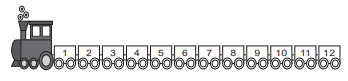
\includegraphics[scale=1.5]{exe1}
\end{figure}

De acordo com as possíveis variações nas colorações dos vagões, a quantidade de trens que pode ser montados, expressa por meio de combinações, é dada por: 

\clearpage
\begin{enumerate}
\item $C^4_{12} \times C^3_{12} \times C^3_{12} \times C^2_{12}$
\item $C^4_{12} + C^3_{8} + C^3_{5} + C^2_{2}$
\item $C^4_{12} \times 2 \times C^3_{8} \times C^2_{5}$
\item $C^4_{12} + 2 \times C^3_{12} \times C^2_{12}$
\item $C^4_{12} \times C^3_{8} \times C^3_{5} \times C^2_{2}$
\end{enumerate}


\item O Salão do Automóvel de São Paulo é um evento no qual vários fabricantes expõe seus modelos mais recentes de veículos, mostrando, principalmente, suas inovações em \textit{design} e tecnologia. 
\begin{flushright}
\small{disponível em http: //g1.globo.com. Acesso em: 4 fev. 2015 (adaptado)}
\end{flushright}

Uma montadora pretende participar desse evento com dois estandes, um na entrada e o outro na região central do salão, expondo, em cada um deles, um carro compacto e uma caminhonete.
Para compor os estandes, foram disponibilizados pela montadora quatro carros compactos, de modelos distintos, e seis caminhonetes de diferentes cores para serem escolhidos aqueles que serão expostos. A posição dos carros dentro de cada estande é irrelevante.
Uma expressão que fornece a quantidade de maneiras diferentes que os estandes podem ser compostos é
 
 \begin{enumerate}
\item $A^4_{10}$
\item $C^4_{10}$
\item $C^2_{4} \times  C^2_{6} \times 2 \times 2$
\item $A^2_{4} \times A^2_{6} \times 2 \times 2$
\item $C^2_{4} \times C^2_{6}$
\end{enumerate}

\item Um brinquedo infantil caminhão-cegonha é formado por uma carreta e dez carrinhos nela transportados, conforme a figura:

\begin{figure}[H]
\centering

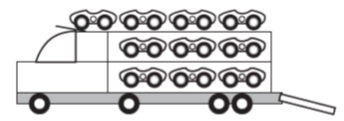
\includegraphics[scale=.75]{exe2}
\end{figure}

No setor de produção da empresa que fabrica esse brinquedo, é feita a pintura de todos os carrinhos para que o aspecto do brinquedo fique mais atraente. São utilizadas as cores amarelo, branco, laranja e verde, e cada carrinho é pintado apenas com uma cor. O caminhão-cegonha tem uma cor fixa. A empresa determinou que em todo caminhão-cegonha deve haver pelo menos um carrinho de cada uma das quatro cores disponíveis. Mudança de posição dos carrinhos no caminhão cegonha não gera um novo modelo do brinquedo.
Com base nessas informações, quantos são os modelos distintos do brinquedo caminhão-cegonha que essa empresa poderá produzir?
 
 \begin{enumerate}
 
\item $C_{6,2}$
\item $C_{9,3}$
\item $C_{10,4}$
\item $6^4$
\item $4^6$
\end{enumerate}

\item (Unesp 2016) Está previsto que, a partir de $1^{o}$ de janeiro de 2017, entrará em vigor um sistema único de emplacamento de veículos para todo o Mercosul, o que inclui o Brasil. As novas placas serão compostas por 4 letras e 3 algarismos. Admita que no novo sistema possam ser usadas todas as 26 letras do alfabeto, incluindo repetições, e os 10 algarismos, também incluindo repetições. Admita ainda que, no novo sistema, cada carro do Mercosul tenha uma sequência diferente de letras e algarismos em qualquer ordem. Veja alguns exemplos das novas placas.

\begin{center}
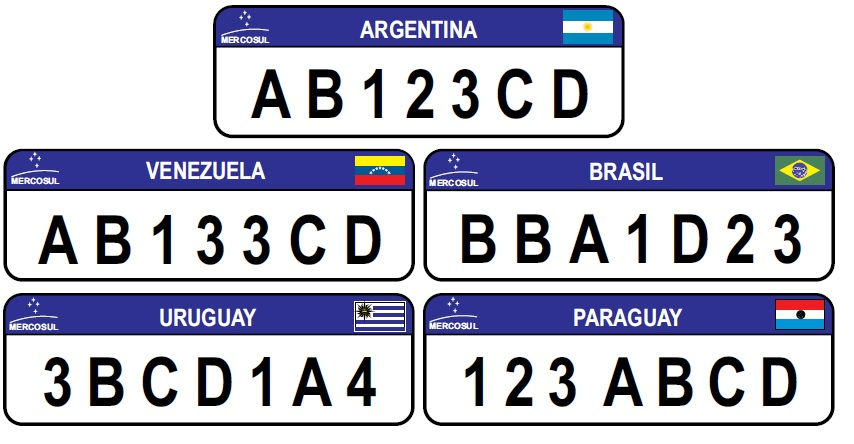
\includegraphics[scale= 0.4]{2f_2016_fig1.jpg}
\end{center}

Imagem: \url{https://drive.google.com/file/d/0Bz49JztKIEhLYmpoVXB6QklMaXc/view}

No novo sistema descrito, calcule o total de placas possíveis com o formato “Letra-Letra-Algarismo-Algarismo–Algarismo-Letra-Letra”, nessa ordem. Em seguida, calcule o total geral de possibilidades de placas com 4 letras (incluindo repetição) e 3 algarismos (incluindo repetição) em qualquer ordem na placa. Deixe suas respostas finais em notação de produto ou de fatorial.

\item Em Hogwarts, uma escola de magia e bruxaria dos filmes e livros de Harry Potter, todos os anos 16 alunos bruxos são divididos em 4 casas, 4 em cada casa, sendo elas: Grifinória, Sonserina, Corvinal e Lufa-Lufa. O personagem principal Harry se torna muito amigo de Rony e os mesmos querem ficar na mesma casa.  Considerando todas as possíveis divisões destes bruxos nas casas, quantas são as chances de Harry e Rony ficarem juntos?

 \item Em Hogwarts, uma escola de magia e bruxaria dos filmes e livros de Harry Potter, todos os anos 16 alunos bruxos são divididos em 4 casas, 4 em cada casa, sendo elas: Grifinória, Sonserina, Corvinal e Lufa-Lufa. O personagem principal Harry não gostaria de estar na mesma casa que  Draco Malfoy. Considerando todas as possíveis divisões destes bruxos nas casas, quantas são as chances de Harry e Malfoy ficarem separados?
\end{enumerate}

\ifnum\aluno=1
\clearpage
\else
\notasfinais
\fi

\bibliographystyle{apalike-pt}
\bibliography{../Bibliografia/combinatoria_bibliografia.bib}

\nocite{*}